%Paul E. West

%\documentclass[xcolor=svgnames]{beamer}
\documentclass{beamer}
\usepackage[boxed,vlined,figure]{algorithm2e}

%\usecolortheme[named=FireBrick]{structure}
%\usecolortheme[named=black]{structure}
%\usecolortheme{beetle}
%\usecolortheme{beaver}
%\usecolortheme{crane}
%\usecolortheme{dolphin}
%\usecolortheme{dove}
%\usecolortheme{fly}
%\usecolortheme{lily}
\usecolortheme{orchid}
%\usecolortheme{rose}
%\setbeamercolor{background canvas}{bg=Gold!25}
%\setbeamercolor{background canvas}{bg=Black!100}
%\setbeamercolor{foreground}{bg=Gold!25}
%\setbeamercolor{normal text}{fg=green,bg=black}
%\setbeamercolor*{palette primary}{use=structure,fg=green,bg=black}

\mode<presentation>{
    \usetheme{Darmstadt}
    \setbeamercovered{invisible}
    %\setbeamercovered{transparent}
    \setbeamercolor*{palette primary}{use=structure,fg=white,bg=blue}
    \setbeamercolor*{palette secondary}{use=structure,fg=white,bg=blue}
    \setbeamercolor*{palette tertiary}{use=structure,fg=white,bg=blue}
}

\usepackage[english]{babel}
\usepackage[latin1]{inputenc}
\usepackage{times}
\usepackage[T1]{fontenc}
%\usepackage{epsfig}
\usepackage{ulem}
\usepackage{color,soul}

\usepackage{graphicx}
\usepackage{amssymb}
\usepackage{url,hyperref}
\definecolor{beamer@blendedblue}{rgb}{1,.6,.2}
%\usepackage{tikz}
%\usetikzlibrary{shapes}
%\usetikzlibrary{arrows}
%\tikzstyle{block}=[draw opacity=0.7, line width=1.4cm]
\usepackage{listings}
\lstset{language=C++}
\lstset{showspaces=false}
\lstset{showstringspaces=false}
\lstset{tabsize=4}
\lstset{basicstyle=\tiny}


%\usecolortheme[overlystylish]{albatross}
%\usecolortheme[]{lily}
%\usecolortheme[]{albatross}
%\usecolortheme[]{orchid}
%\setbeamercolor{normal text}{fg=green!10}

\title{CSCI 315: Data Structures \\ Performance Analysis}
\author{Paul E. West, PhD}

\institute{
  Department of Computer Science\\
  Charleston Southern University
}

\subject{Software Programming}
%\keywords{Performance Counters, Multicore}

%\pgfdeclareimage[height=1.0cm]{university-logo}{../imgs/csu-logo}
\pgfdeclareimage[height=0.75cm]{university-logo}{../imgs/csu-logo}
%\pgfdeclareimage[height=0.50cm]{university-logo}{../imgs/csu-logo}
\logo{\pgfuseimage{university-logo}}

\begin{document}

\begin{frame}
  \titlepage
\end{frame}

\section{Intro}
\subsection{}


\begin{frame}{Analysis of Algorithms}
\begin{itemize}
\item Dilemma:  you have two (or more) methods to solve problem, how to choose the BEST?
\item One approach: implement each algorithm in C, test how long each takes to run.
\item Problems:
\begin{itemize}
\item Different implementations may cause an algorithm to run faster/slower
\item Some algorithms run faster on some computers
\item Algorithms may perform differently depending on data (e.g., sorting often depends on what is being sorted)
\end{itemize}
\end{itemize}
\end{frame}

\begin{frame}{Better Approach Step 1}
\begin{itemize}
\item characterize performance in terms of key operation(s)
\item Sorting:
\begin{itemize}
\item count number of times two values compared
\item count number of times two values swapped
\end{itemize}
\item Search:
\begin{itemize}
\item count number of times value being searched for is compared to values in array
\end{itemize}
\item Recursive function:
\begin{itemize}
\item count number of recursive calls
\end{itemize}
\end{itemize}
\end{frame}

%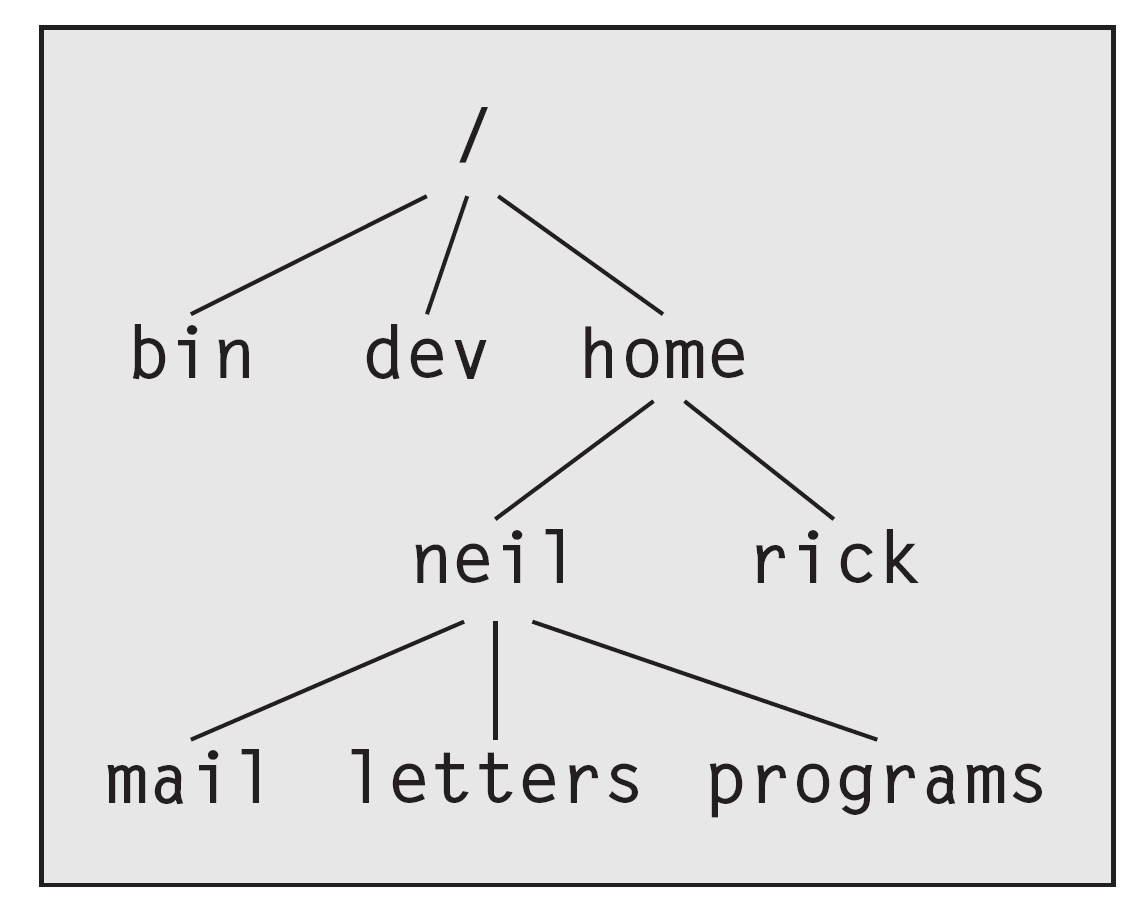
\includegraphics[width=1.0\textwidth]{../imgs/simple-directories.png}
\begin{frame}{Better Approach Step 2}
\begin{itemize}
\item Want to comment on the ``general'' performance of the algorithm
\item Emperical: Measure for several examples, but what does this tell us in general?
\item Analytical:
\begin{itemize}
\item Instead, assess performance in an abstract manner
\item Idea: analyze performance as size of problem grows
\item Examples:
\begin{itemize}
\item Sorting: how many comparisons for array of size N?
\item Searching: \#comparisons for array of size N
\end{itemize}
\item May be difficult to discover a reasonable formula
\end{itemize}
\end{itemize}
\end{frame}

%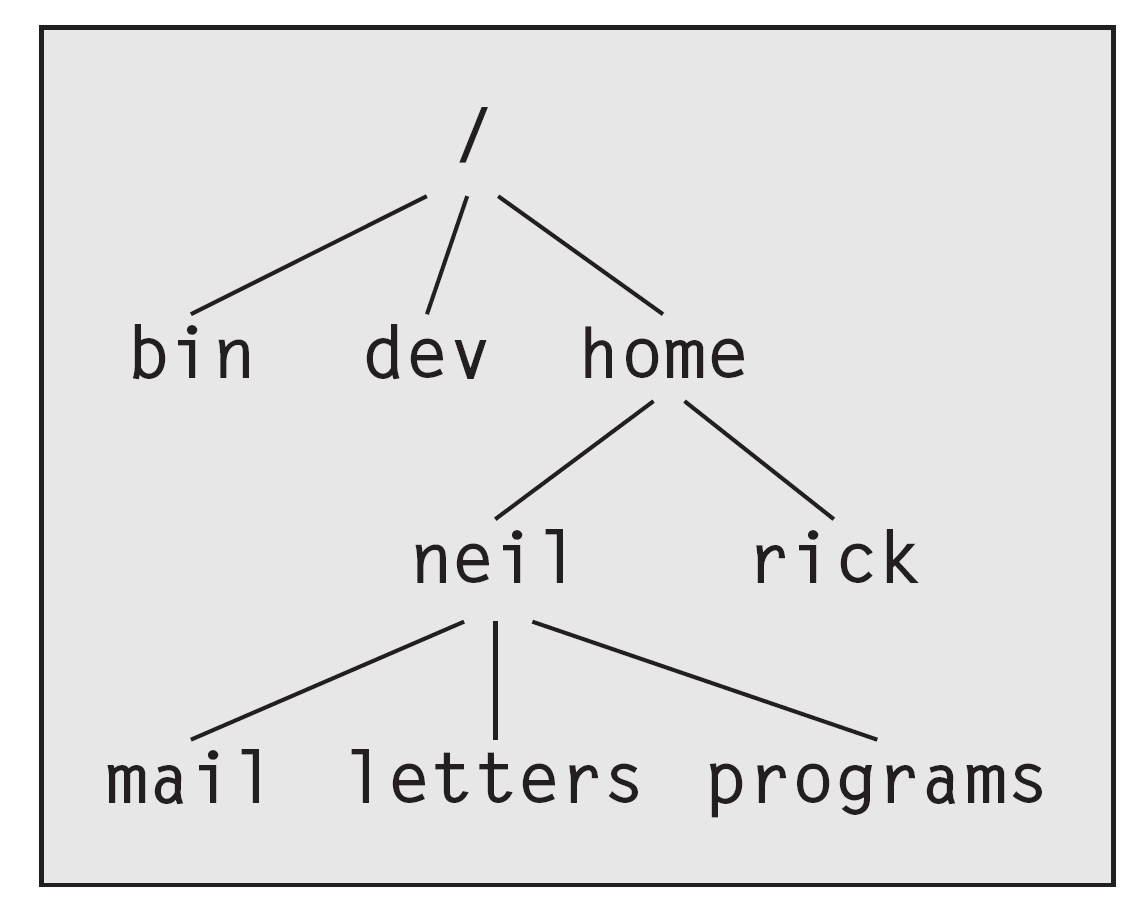
\includegraphics[width=1.0\textwidth]{../imgs/simple-directories.png}
\begin{frame}{Analsysis With Varying Results}
\begin{itemize}
\item Example: for some sorting algorithms, a sorting routine may require as few as N-1 comparisons and as many as $\frac{N^2}{2}$
\item Types of analyses:
\begin{itemize}
\item Best-case: what is the fastest an algorithm can run for a problem of size N?
\item Average-case: on average how fast does an algorithm run for a problem of size N?
\item Worst-case: what is the longest an algorithm can run for a problem of size N?
\end{itemize}
\item Computer scientists \textit{usually} use worst-case analysis
\end{itemize}
\end{frame}

%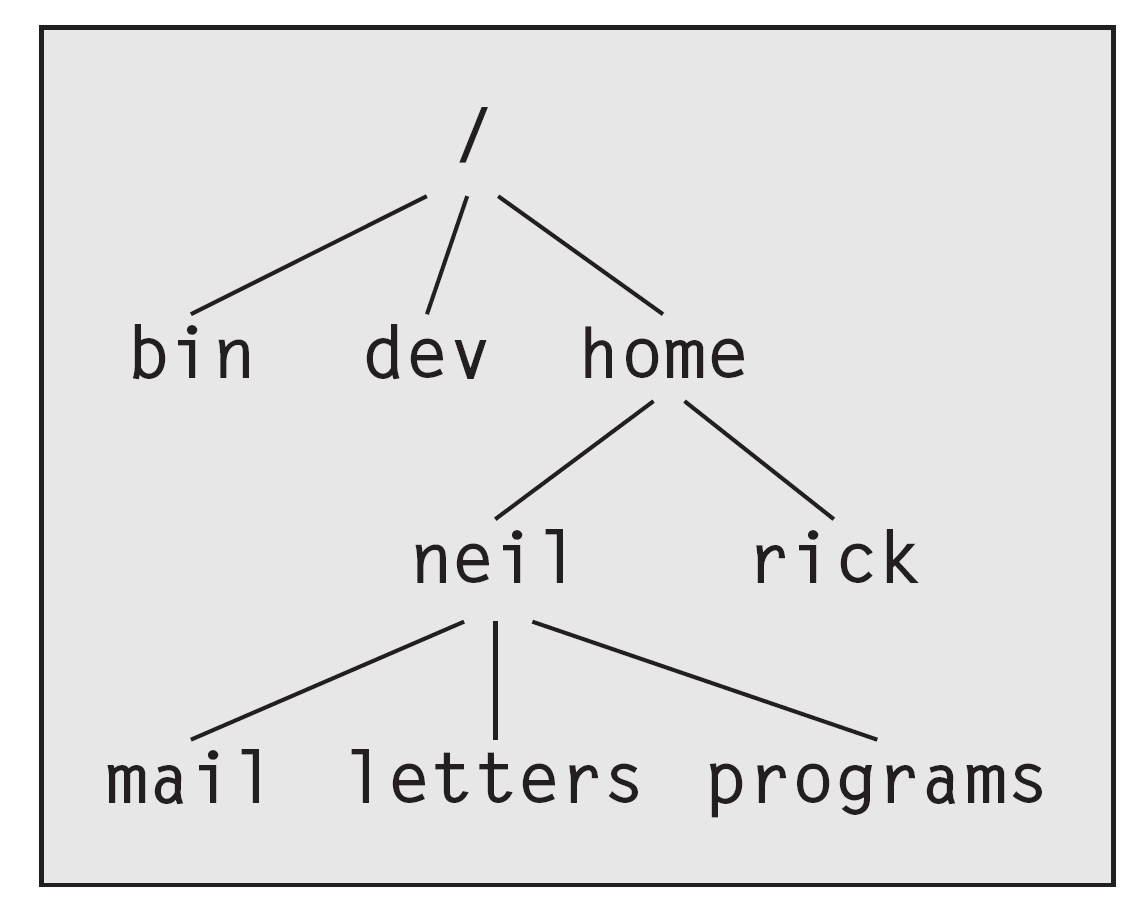
\includegraphics[width=1.0\textwidth]{../imgs/simple-directories.png}
\begin{frame}{Notice: We Are \textbf{Estimating}}
\begin{itemize}
\item What is often done is to approximate or estimate the performance of an algorithm
\item Estimation is an important skill to learn and to use
\item Example Question: How many hotdogs tall is the Empire State Building?
\end{itemize}
\end{frame}

%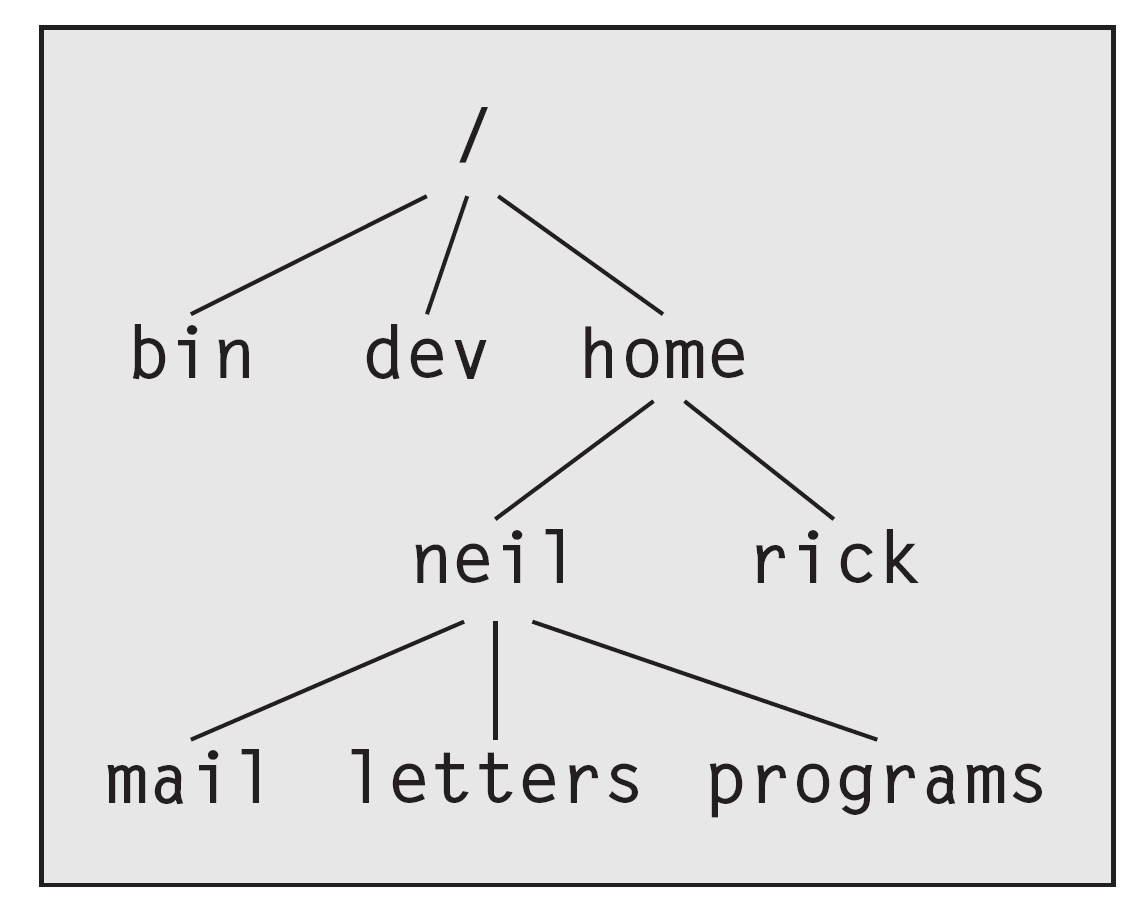
\includegraphics[width=1.0\textwidth]{../imgs/simple-directories.png}
\begin{frame}{Simple Example}
\begin{columns}
\column{0.50\textwidth}
\begin{itemize}
\item Simplier Question: How tall is the Empire State Building?
\item Answer: The ESB is 1250 feet tall.
\item Assuming that a hotdog is 6 inches from end to end, you would need, 1250 * 2 = 2500 hotdogs.
\end{itemize}
\column{0.50\textwidth}
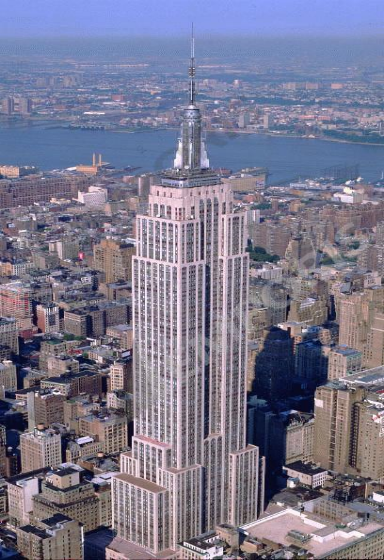
\includegraphics[width=0.9\textwidth]{../imgs/empire-state.png}
\end{columns}
\end{frame}

\section{Complexity Analysis}
\subsection{}
%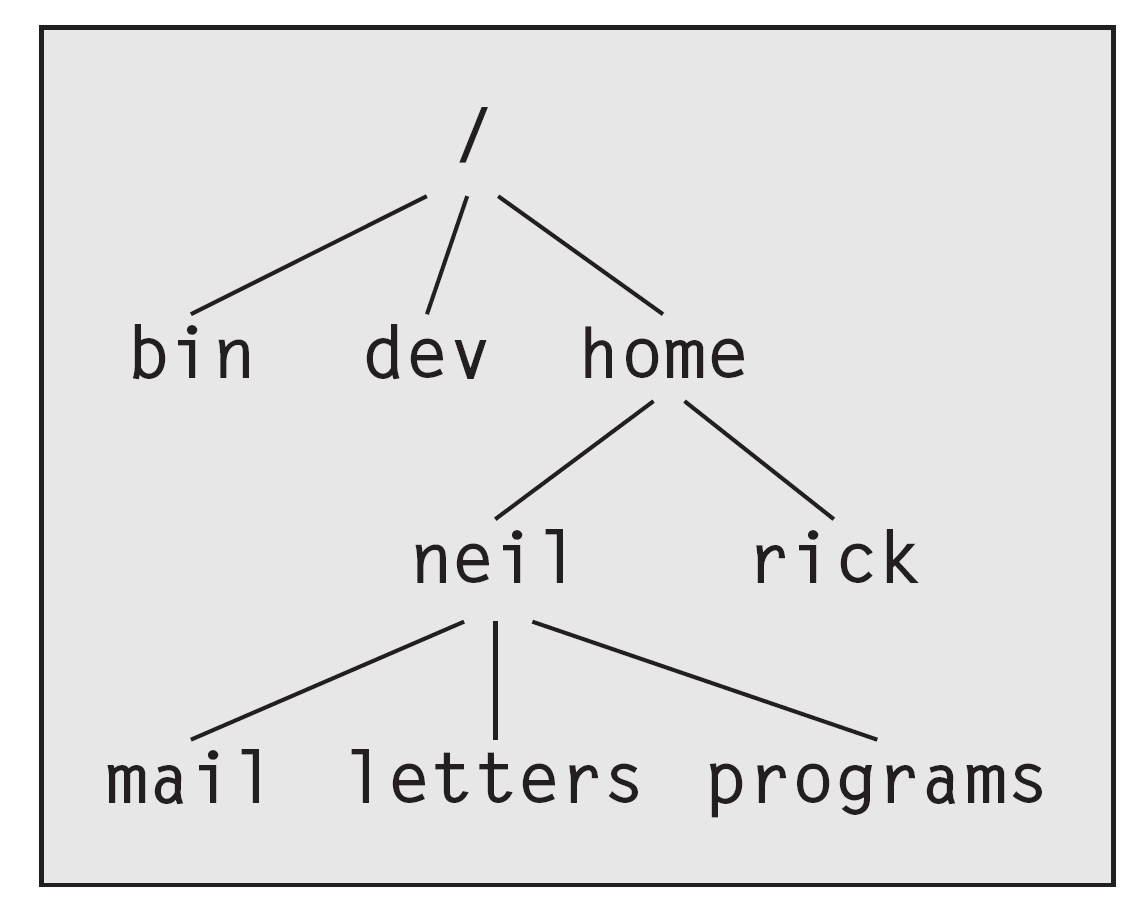
\includegraphics[width=1.0\textwidth]{../imgs/simple-directories.png}
\begin{frame}{Analysis}
\begin{itemize}
\item An objective way to evaluate the cost of an algorithm or code section.  
\item The cost is computed in terms of space or time, usually
\item The goal is to have a meaningful way to compare algorithms based on a common measure.
\item Complexity analysis has two phases,
\begin{itemize}
\item Algorithm analysis
\item Complexity analysis
\end{itemize}
\end{itemize}
\end{frame}

%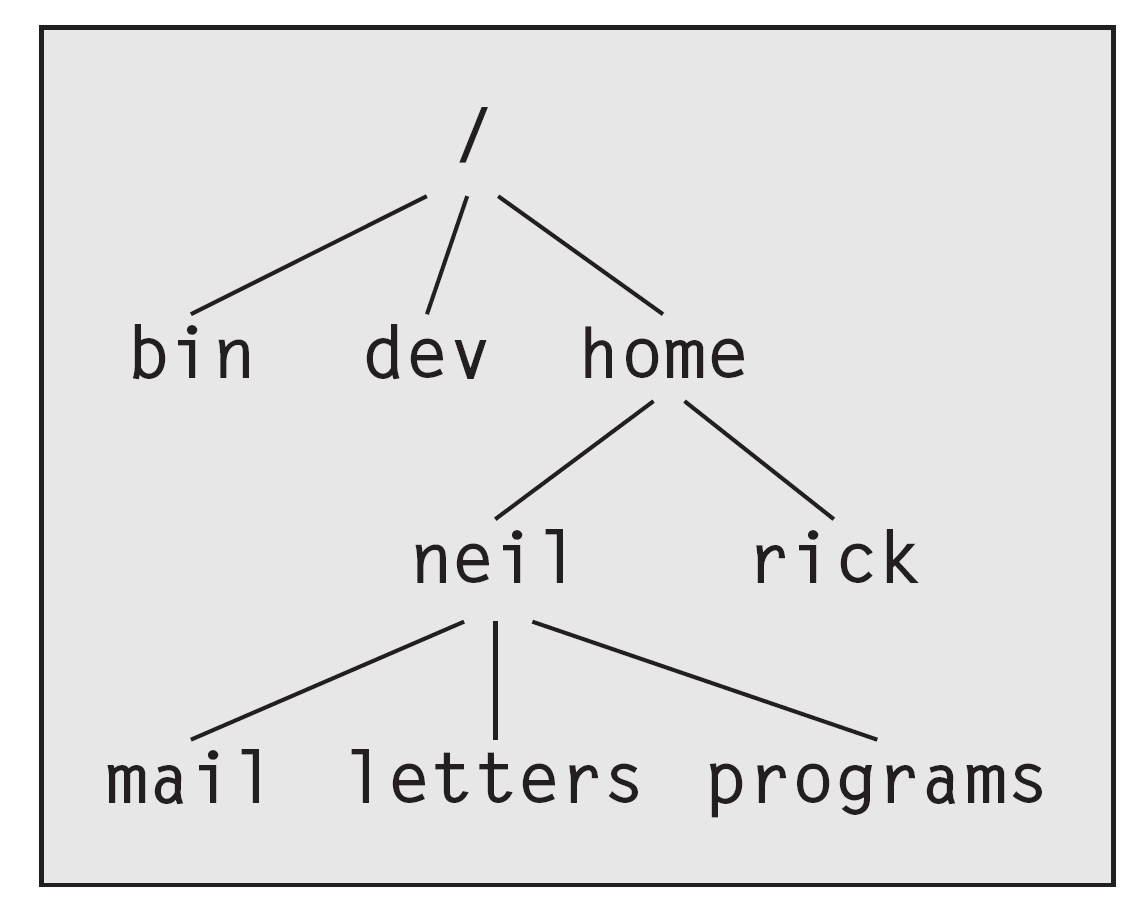
\includegraphics[width=1.0\textwidth]{../imgs/simple-directories.png}
\begin{frame}{Algorithm Analysis}
\begin{itemize}
\item Algorithm analysis requires a set of rules to determine how operations are to be counted.
\item There is no generally accepted set of rules for algorithm analysis.
\item In some cases, an exact count of operations is desired; in other cases, a general approximation is sufficient.
\item The rules presented that follow are typical of those intended to produce an exact count of operations.
\end{itemize}
\end{frame}

%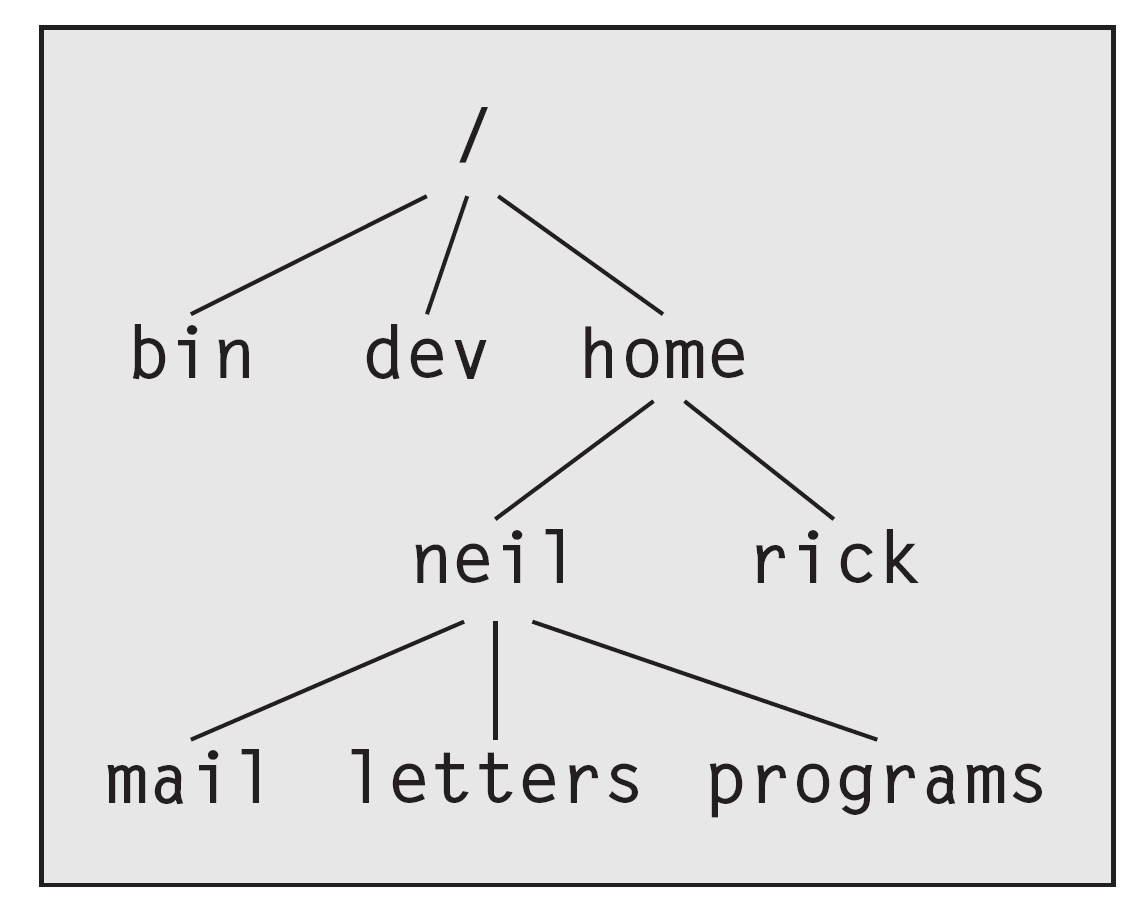
\includegraphics[width=1.0\textwidth]{../imgs/simple-directories.png}
\begin{frame}{Rules}
\begin{enumerate}
\item We assume an arbitrary time unit.
\item Execution of one of the following operations takes time 1:
\begin{enumerate}
\item assignment operation
\item single I/O operations
\item single Boolean operations, numeric comparisons
\item single arithmetic operations
\item function return
\item array index operations, pointer dereferences
\end{enumerate}
\end{enumerate}
\end{frame}

%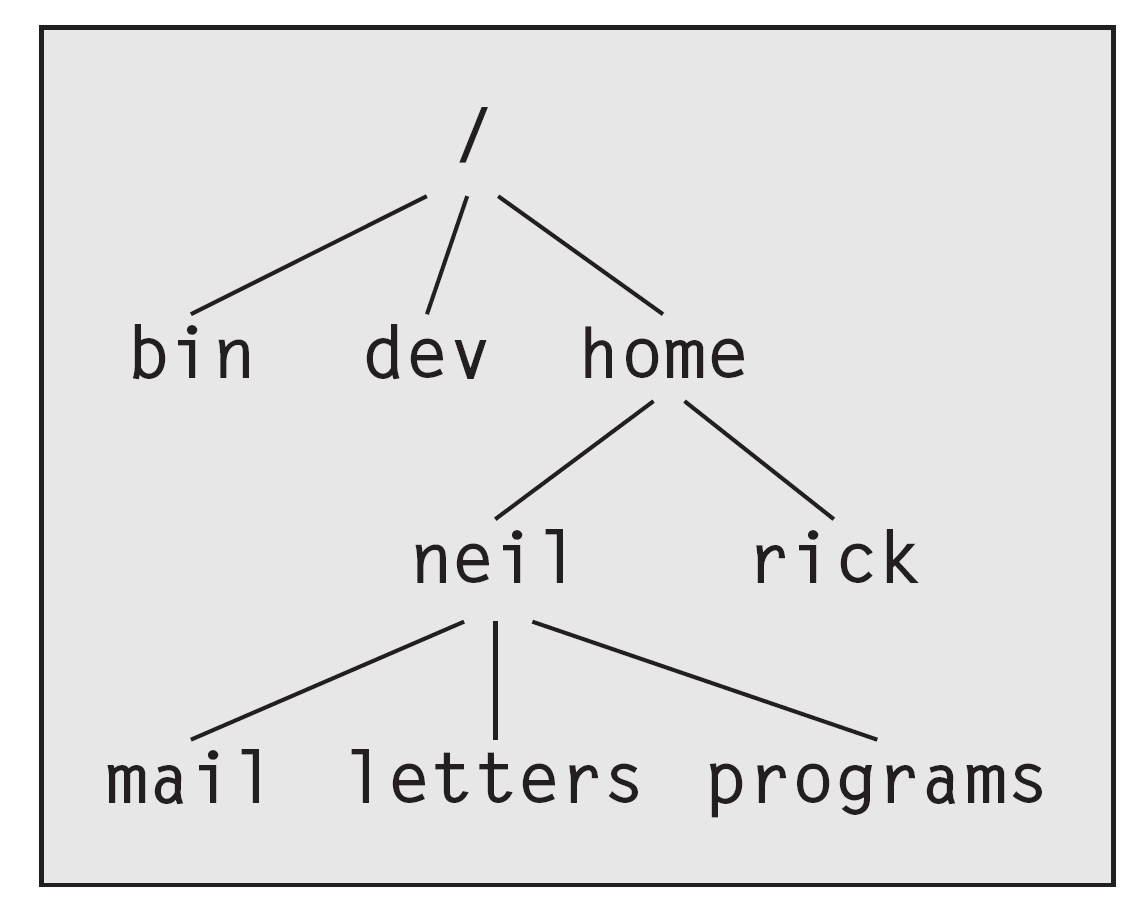
\includegraphics[width=1.0\textwidth]{../imgs/simple-directories.png}
\begin{frame}{More Rules}
\begin{enumerate}
\setcounter{enumi}{2}
\item Running time of a selection statement (if, switch) is the time for the condition evaluation + the maximum of the running times for the individual clauses in the selection.
\item Loop execution time is the sum, over the number of times the loop is executed, of the body time + time for the loop check and update operations, + time for the loop setup.
\item Always assume that the loop executes the maximum number of iterations possible
Running time of a function call is 1 for setup + the time for any parameter calculations + the time required for the execution of the function body.
\end{enumerate}
\end{frame}

%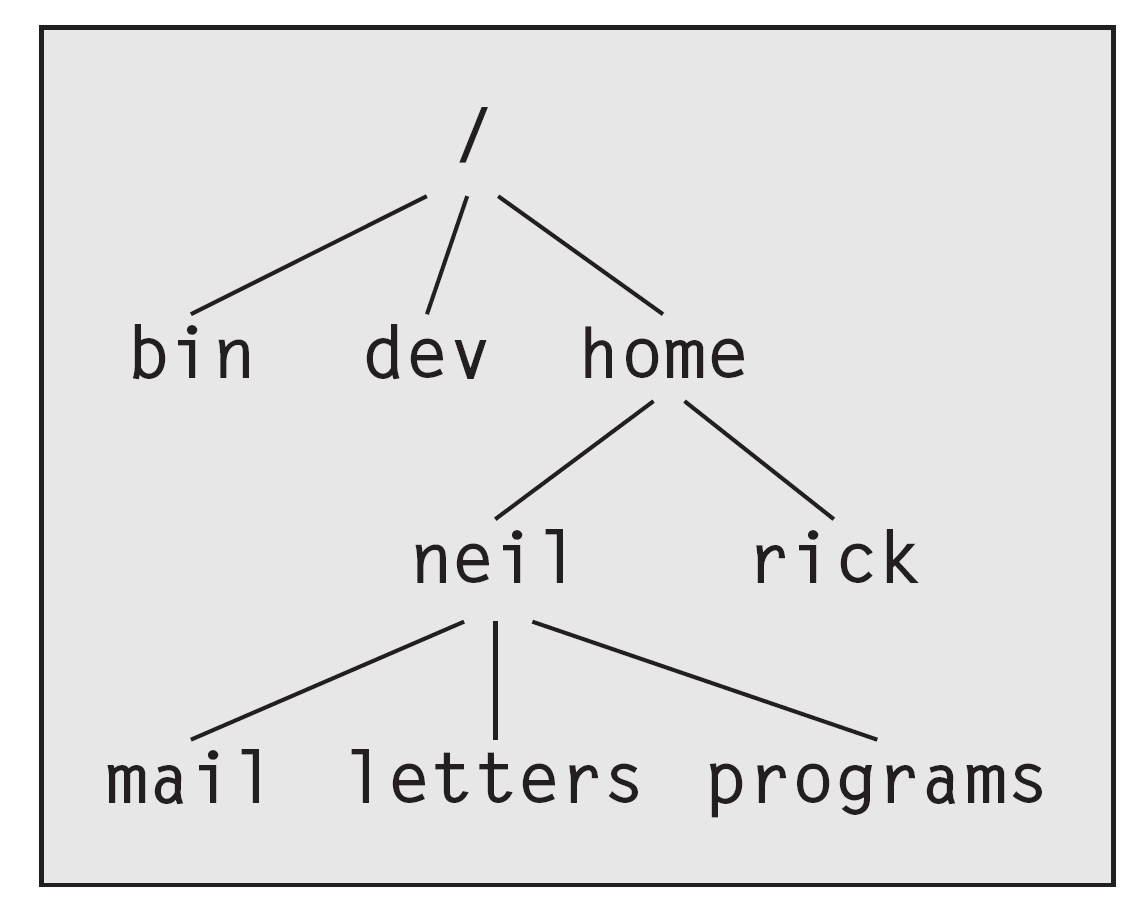
\includegraphics[width=1.0\textwidth]{../imgs/simple-directories.png}
\begin{frame}[fragile]{Example 1}
\begin{lstlisting}
count = count + 1;  // Cost: c1
sum = sum + count;  // Cost: c2 
\end{lstlisting}
Total Cost = c1 + c2. \\
Since we assume '+' cost 1 and assignment cost 1, the total cost is 4.
\end{frame}

\begin{frame}[fragile]{Example 2}
\begin{lstlisting}
if (n < 0) { // Cost: c1
    absval = -n; // Cost: c2
} else {
    absval = n; // Cost: c3
}

\end{lstlisting}
\begin{itemize}
\item Total Cost  <=  c1 + max(c2,c3)
\item c1 is the cost of boolean evaluation.  Since there is 1 evaluation ($<$), Cost(c1) = 1.
\item c2 is the cost of negating a number (1) + the cost of assignment (1).  Cost(c2) = 2.
\item c3 is the cost of assignment(1).  Cost(c3) = 1
\item Cost of the worse-case is 3.
\item Cost of the best-cast is 2.
\item Average case is 2.5.
\end{itemize}
\end{frame}

\begin{frame}[fragile]{Example 3}
\begin{lstlisting}
    i = 1; // Cost: c1
    sum = 0; // Cost: c2
    while (i <= n) { // Cost: c3
        i = i + 1; // Cost: c4
        sum = sum + i; // Cost: c5
    } 
\end{lstlisting}
\begin{itemize}
\item <2-> Cost(c1) = 1, Cost(c2) = 1, Cost(c3) = 1.
\item <3-> Cost(c4) = 1 + 1 = 2 (remember assignment and + both cost 1!).
\item <4-> Cost(c5) = 2.
\item <5-> How many time does the loop execute?
\item <6-> Loop: n times, so total cost is:
\item <7-> Total Cost = c1 + c2 + (n+1)*c3 + n*c4 + n*c5 = \\
c1 + c2 + c3 + n(c3 + c4 + c5)
\end{itemize}
\end{frame}

\begin{frame}[fragile]{Nested Example}
\begin{lstlisting}
i = 1; // Cost c1
sum = 0;  // Cost c2
while (i <= n) {  // Cost c3
    j = 1; // Cost c4
    while (j <= n) { // Cost c5
        sum = sum + i; // Cost c6
        j = j + 1;   // Cost c7
    }
    i = i + 1; // Cost c8
}
\end{lstlisting}
\begin{itemize}
\item <2-> Cost(c1) = 1, Cost(c2) = 1, Cost(c3) = 1, Cost(c4) = 1, Cost(c5) = 1, Cost(c6) = 2, Cost(c7) = 2, Cost(c8) = 2
\item <3-> First (outer) while loop execution: n
\item <4-> Second (inner) while loop execution: n, total cost is: \\
\item <5->{\tiny $c1 + c2 + (n+1)*c3 + n*c4 + n*(n+1)*c5+n*n*c6+n*n*c7+n*c8 = $\\
$c1 + c2 + c3 + n*(c3 + c4 + c8) + n*n*c5 + n*c5 + n*n*c6+n*n*c7 = $\\
$c1 + c2 + c3 + n*(c3 + c4 + c5 + c8) + n*n(c5 + c6 + c7)$ }
\item <6-> \textbf{Important Note:} n*n ($n^2$) is the highest (largest) term!
\end{itemize}
\end{frame}

\section{Big O}
\subsection{}

\begin{frame}{Comparing Algorithms}
\begin{itemize}
\item We measure an algorithm's time requirement as a function of the problem size.
\item Problem size depends on the application: e.g. number of elements in a list for a sorting algorithm, the number disks for towers of hanoi.
\item So, for instance, we say that (if the problem size is n)
\begin{itemize}
\item Algorithm A requires $5*n^2$ time units to solve a problem of size n.
\item Algorithm B requires $7*n$  time units to solve a problem of size n.
\end{itemize}
\item An algorithm's proportional time requirement is known as growth rate.
\item We can compare the efficiency of two algorithms by comparing their growth rates.
\end{itemize}
\end{frame}

\begin{frame}{Example}
\begin{itemize}
\item Which is better?
\begin{itemize}
\item $50N^2 + 31N^3 + 24N + 15$
\item $3N^2 + N + 21 + 4*3^N$
\end{itemize}
\item <2-> Well, it depends on N: \\
\begin{tabular}{l l l}
N  & $50N^2 + 31N^3 + 24N + 15$ & $3N^2 + N + 21 + 4*3^N$ \\
1   &       120     &           37 \\
2   &       511     &           71 \\
3   &      1374     &          159 \\
4   &      2895     &          397 \\
5   &      5260     &         1073 \\
6   &      8655     &         3051 \\
7   &     13266     &         8923 \\
8   &     19279     &        26465 \\
9   &     26880     &        79005 \\
10  &     36255     &       236527 \\
\end{tabular}
\end{itemize}
\end{frame}

\begin{frame}{What happened?}

\begin{tabular}{l l l l}
N  & $3N^2 + N + 21 + 4*3^N$  & $4*3^N$ & \% of Total \\
1  &         37  &        12  &      32.4 \\
2  &         71  &        36  &      50.7 \\
3  &        159  &       108  &      67.9 \\
4  &        397  &       324  &      81.6 \\
5  &       1073  &       972  &      90.6 \\
6  &       3051  &      2916  &      95.6 \\
7  &       8923  &      8748  &      98.0 \\
8  &      26465  &     26244  &      99.2 \\
9  &      79005  &     78732  &      99.7 \\
10 &     236527  &    236196  &      99.9 \\
\end{tabular}

\begin{itemize}
\item One term dominated the others.
\item This implies we \textit{really} only care about the dominating (highest/largest) term.
\end{itemize}
\end{frame}

\begin{frame}{As N Grows, Some Terms Dominate}
\begin{tabular}{l l l l l l}
Function   & N=10   & N=100  & N=1000 & N=10000 & N = 100000 \\
$log_2N$   & 3      & 6      & 9      & 13      & 16 \\
$N$        & 10     & 100    & 1000   & 10000   & 100000 \\
$N*log_2N$ & 30     & 664    & 9965   & $10^5$  & $10^6$ \\
$N^2$      & $10^2$ & $10^4$ & $10^6$ & $10^8$  & $10^{10}$ \\
$N^3$      & $10^3$ & $10^6$ & $10^9$ & $10^{12}$  & $10^{15}$ \\
$2^N$      & $10^3$ & $10^{30}$ & $10^{301}$ & $10^{3010}$  & $10^{30103}$ \\
\end{tabular}
\begin{itemize}
\item Ordering:\\
$1 < log_2N < N < N*log_2N < N^2 < N^3 < 2^N < 3^N$
\end{itemize}
\end{frame}

%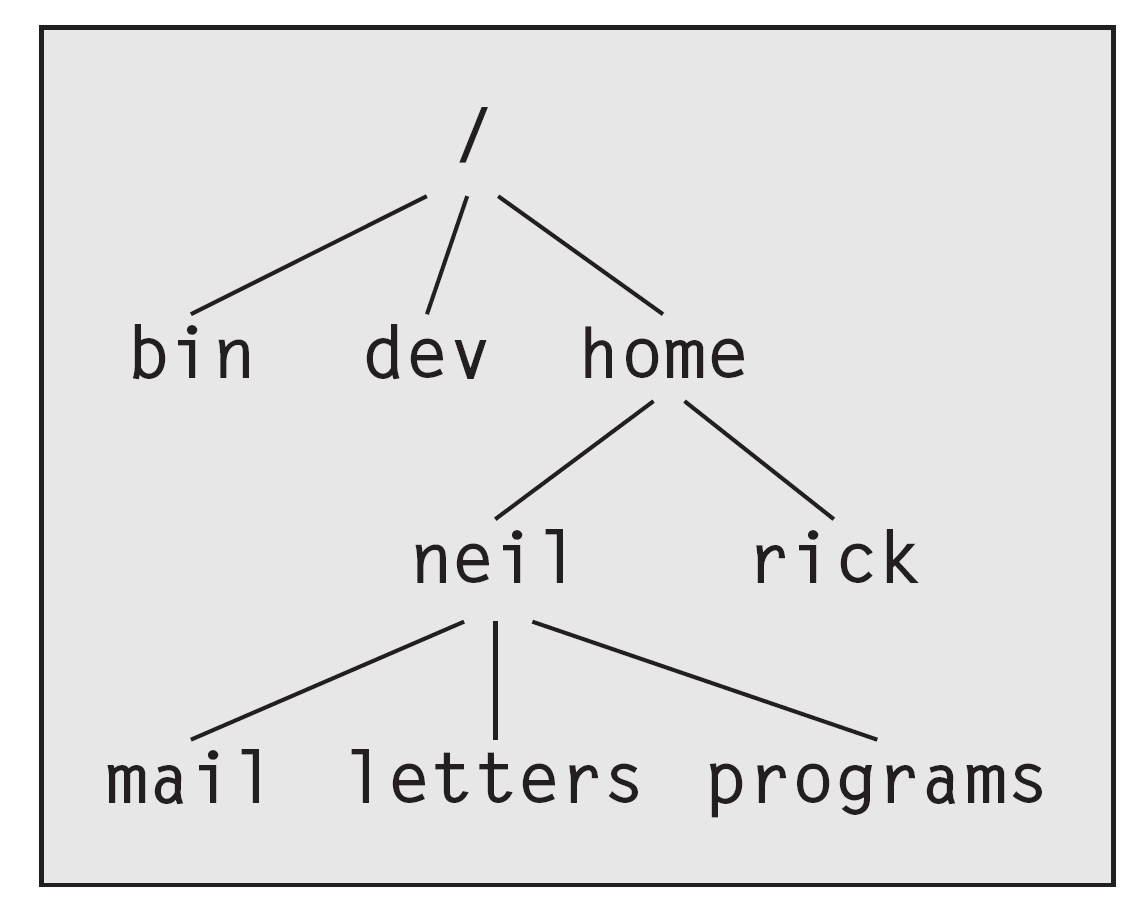
\includegraphics[width=1.0\textwidth]{../imgs/simple-directories.png}
\begin{frame}{Big O}
\begin{itemize}
\item If  Algorithm A requires time proportional to $f(n)$, Algorithm A is said to be order $f(n)$, and it is denoted as $O(f(n))$.
\item The function $f(n)$ is called the algorithm's growth-rate function.
\item Since the capital O is used in the notation,  this notation is called the Big O notation.
\item If Algorithm A requires time proportional to $n^2$, it is $O(n2)$.
\item If Algorithm A requires time proportional to $n$, it is $O(n)$.
\end{itemize}
\end{frame}

%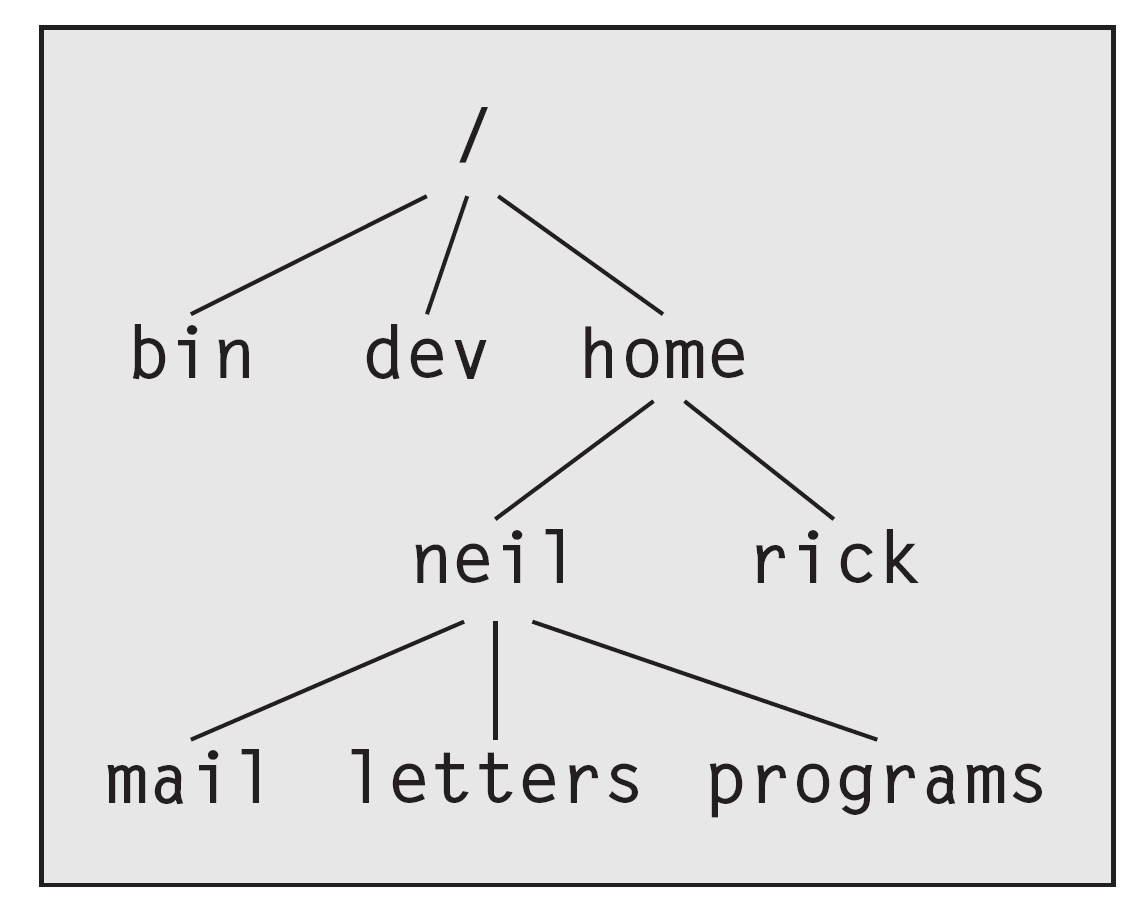
\includegraphics[width=1.0\textwidth]{../imgs/simple-directories.png}
\begin{frame}{Example 1}
\begin{itemize}
\item If an algorithm requires $n^2-3*n+10$ seconds to solve a problem size n. If constants $k$ and $n_0$ exist such that \\
$k*n^2 + n_0 > n^2-3*n+10$ for all $n$ and $n_0$.
\item Then the algorithm is order $n^2$  (In fact, $k$ is 3 and $n_0$ is 2)
\item Thus, the algorithm requires no more than $k*n^2$ time units.
\item So it is $O(n^2)$
\end{itemize}
\end{frame}

%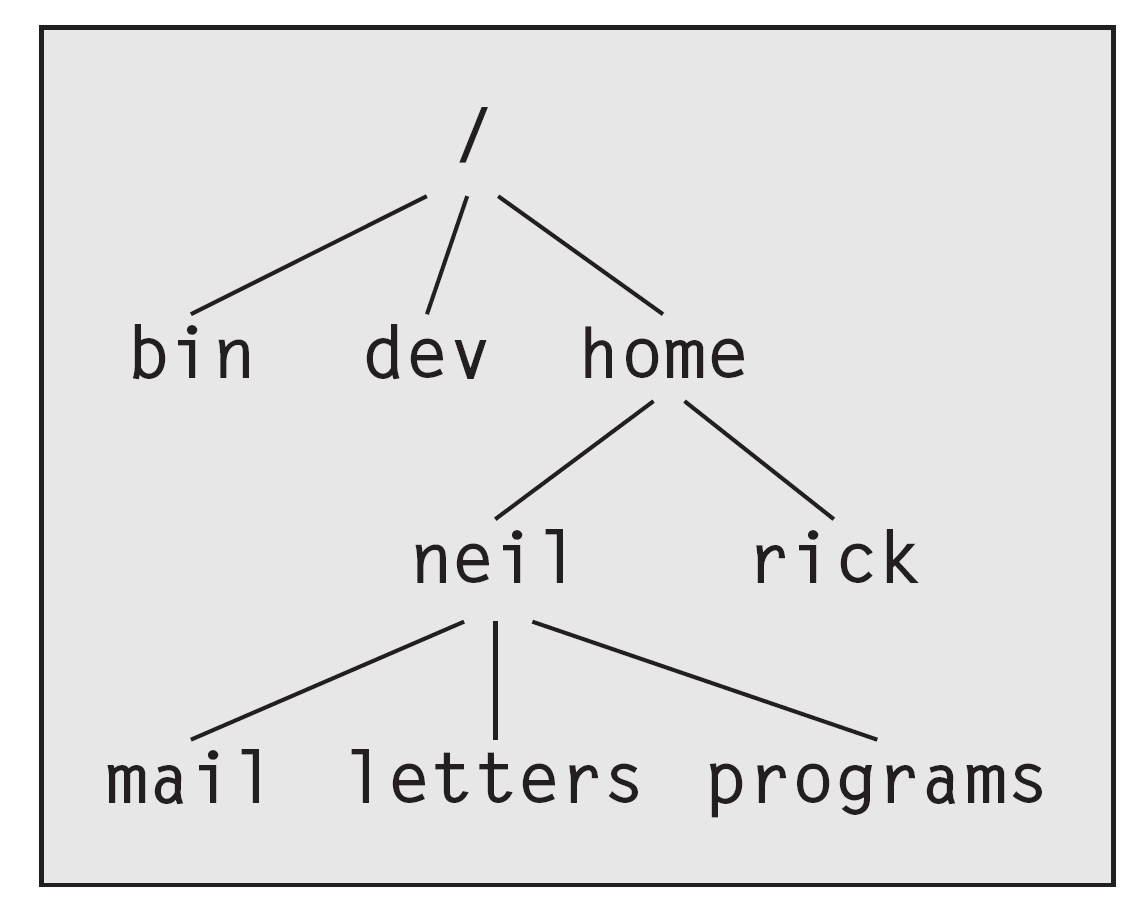
\includegraphics[width=1.0\textwidth]{../imgs/simple-directories.png}
\begin{frame}{Examples}
\begin{itemize}
\item This is actually not that difficult.  It is a game of ``spot the highest term!''
\item $50N^2 + 31N^3 + 24N + 15$ = $O(N^3)$ 
\item $3N^2 + N + 21 + 4*3^N$  = $O(3^N)$
\item It can get somewhat tricky:
\item $N(3 + N(9+N)) + N^2$ = $O(N^3)$
\item $N(10 + log_2N) + N$ = $O(N*log_2N)$
\end{itemize}
\end{frame}

%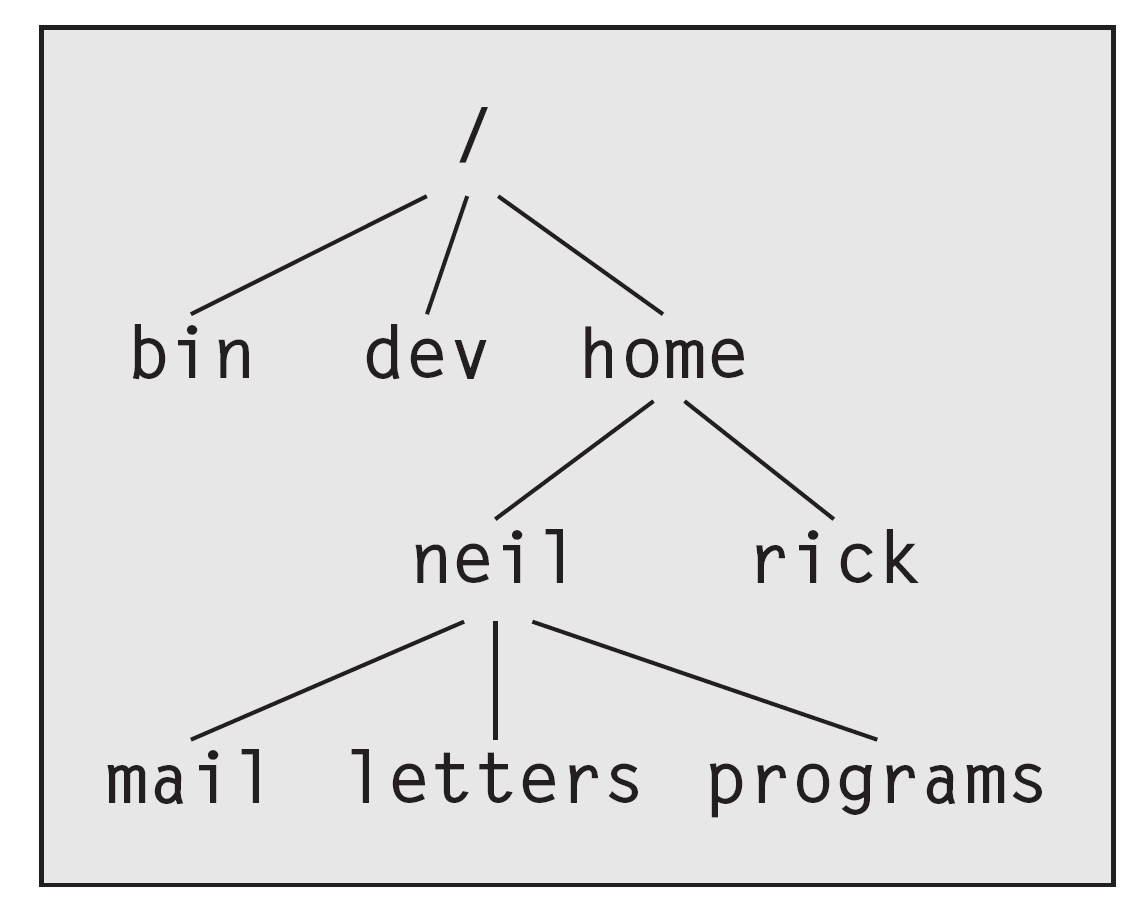
\includegraphics[width=1.0\textwidth]{../imgs/simple-directories.png}
\begin{frame}{Growth Reate Function Explained}
\begin{itemize}
\item $O(1)$             Time requirement is constant, and it is independent of the problem's size.
\item $O(log_2n)$      Time requirement for a logarithmic algorithm increases increases slowly
                 as the problem size increases.
\item $O(n)$      Time requirement for a linear algorithm increases directly with the size
                 of the problem.
\item $O(n*log_2n)$ Time requirement for a $n*log_2n$ algorithm increases more rapidly than
                 a linear algorithm.
\item $O(n^2)$       Time requirement for a quadratic algorithm increases rapidly with the
                 size of the problem.
\item $O(n^3)$       Time requirement for a cubic algorithm increases more rapidly with the
                 size of the problem than the time requirement for a quadratic algorithm.
\item $O(2^n)$      As the size of the problem increases, the time requirement is too rapid to be practical.
\end{itemize}
\end{frame}

\section{Practice}
\subsection{}
\begin{frame}[fragile]{Example 1}
\begin{lstlisting}
i = 1; // Cost c1
sum = 0; // Cost c2
while (i <= n) { // Cost c3
    i = i + 1; // Cost c4
    sum = sum + i; // Cost c5
} 
\end{lstlisting}
\begin{itemize}
\item <2-> T(n)  =  c1 + c2 + (n+1)*c3 + n*c4 + n*c5 \\
            = (c3+c4+c5)*n + (c1+c2+c3) \\
            = a*n + b
\item <2-> So, the growth-rate function for this algorithm is $O(n)$
\end{itemize}
\end{frame}

\begin{frame}[fragile]{Example 2}
\begin{lstlisting}
i=1; // Cost c1
sum = 0;  // Cost c2
while (i <= n) {  // Cost c3
    j=1; // Cost c4
    while (j <= n) { // Cost c5
        sum = sum + i; // Cost c6
        j = j + 1;  // Cost c7
    }
    i = i +1 // Cost c8
}
\end{lstlisting}
\begin{itemize}
\item <2-> T(n)  =  c1 + c2 + (n+1)*c3 + n*c4 + n*(n+1)*c5+n*n*c6+n*n*c7+n*c8 \\
            = (c5+c6+c7)*n*n + (c3+c4+c5+c8)*n + (c1+c2+c3) \\
            = a*n*n + b*n + c \\
\item <2-> So, the growth-rate function for this algorithm is $O(n^2)$
\end{itemize}
\end{frame}

\begin{frame}[fragile]{Example 3}
\begin{lstlisting}
for (i=1; i<=n; i++) { // Cost(c1)
    for (j=1; j<=i; j++) { // Cost(c2)
        for (k=1; k<=j; k++) { // Cost(c3)
            x=x+1; // Cost(c4)
        }
    }
}
\end{lstlisting}
\begin{itemize}
\item <2-> T(n)  =  c1*(n+1) + c2*((n+1)*(n+2)) / 2) + c3* ( estimated: (n * (n + 1) * (2n + 1)) / 6) + c4*( estimated: (n * (n + 1) * (2n + 1)) / 6) \\
            = a*n3 + b*n2 + c*n + d
\item <2-> So, the growth-rate function for this algorithm is $O(n^3)$
\item <2-> \textbf{Notice:} You do NOT need to know the exact number of iterations to find Big-O.
\end{itemize}
\end{frame}

%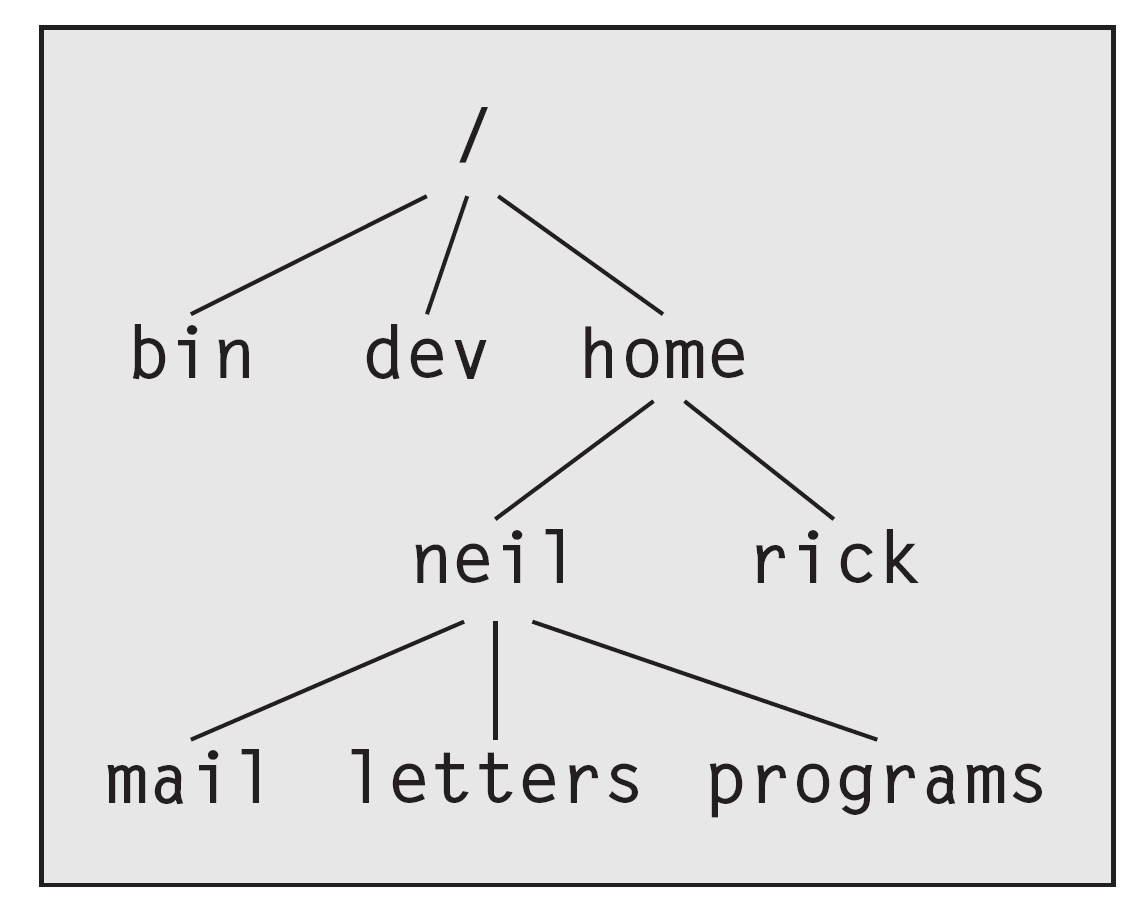
\includegraphics[width=1.0\textwidth]{../imgs/simple-directories.png}
\begin{frame}[fragile]{Example 4}
Unfortunately, recursive can be hard...
\begin{lstlisting}
void hanoi(int n, char source, char dest, char spare) { // Cost of function call
  if (n > 0) { // Cost(c1)
       hanoi(n-1, source, spare, dest);  // Cost(c2)
    cout << "Move top disk from pole " << source
              << " to pole " << dest << endl; // Cost(c3)
       hanoi(n-1, spare, dest, source);  // Cost(c4)
} }
\end{lstlisting}
\begin{itemize}
\item By now, I hope you see that constance costs are virtually supurfulous when working with Big O.
\item To find the growth-rate function for a recursive algorithm, we have to solve its recurrence relation.
\item You will learn how to do this in Discrete Structures.
\end{itemize}
\end{frame}

%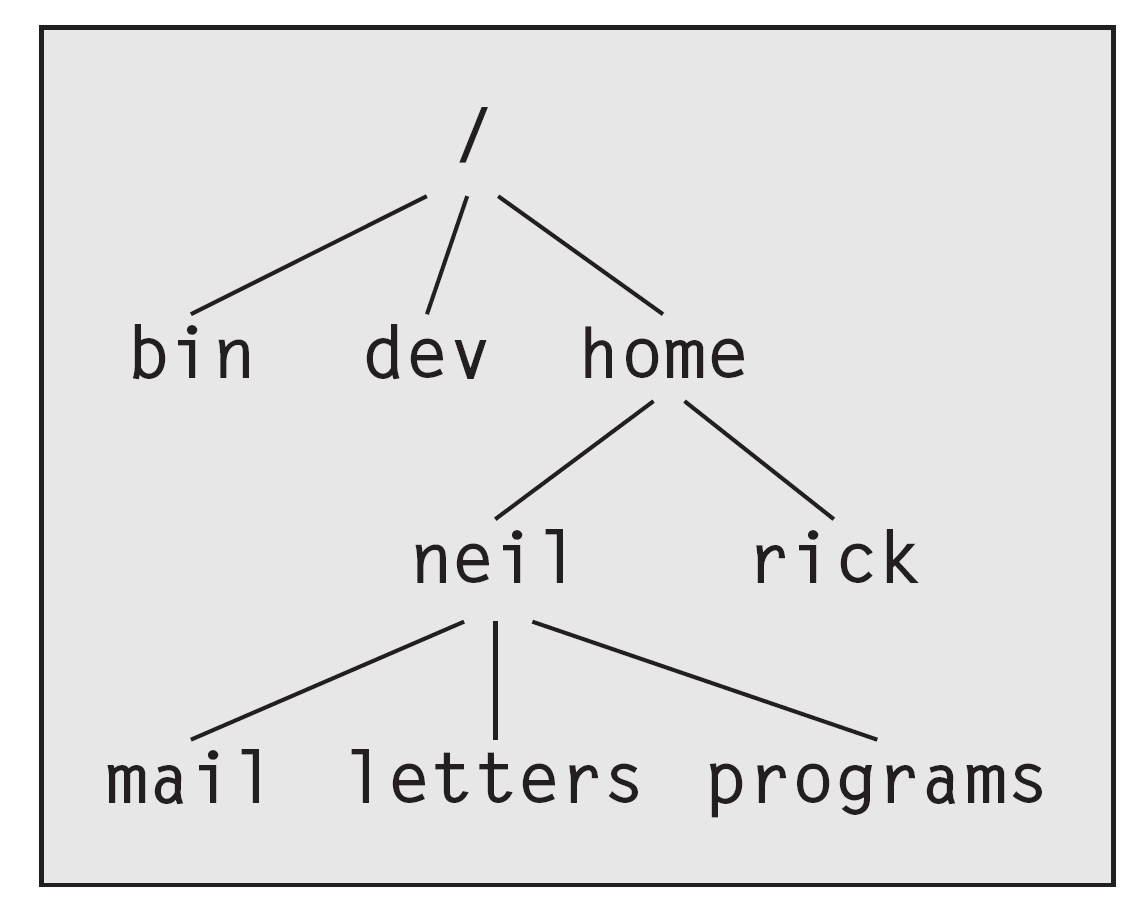
\includegraphics[width=1.0\textwidth]{../imgs/simple-directories.png}
\begin{frame}{Example 4 continued}
\begin{itemize}
\item What is the cost of hanoi(n,'A','B','C')?
\item when n=0
      T(0) = c1 
\item when n>0
      T(n) = c1 + c2 + T(n-1) + c3 + c4 + T(n-1) \\
           = 2*T(n-1) + (c1+c2+c3+c4) \\
           = 2*T(n-1) + c   -> recurrence equation for the growth-rate function of hanoi-towers algorithm  \\
\item Now, we have to solve this recurrence equation to find the growth-rate function of hanoi-towers algorithm
\item This turns out to be $O(2^n)$ because for every N we make 2(n-1) calls.
\end{itemize}
\end{frame}

%http://academic.regis.edu/dbahr/GeneralPages/DataStructures/DataStrucPart4.pdf

%\section{gprof}
%\subsection{}
%%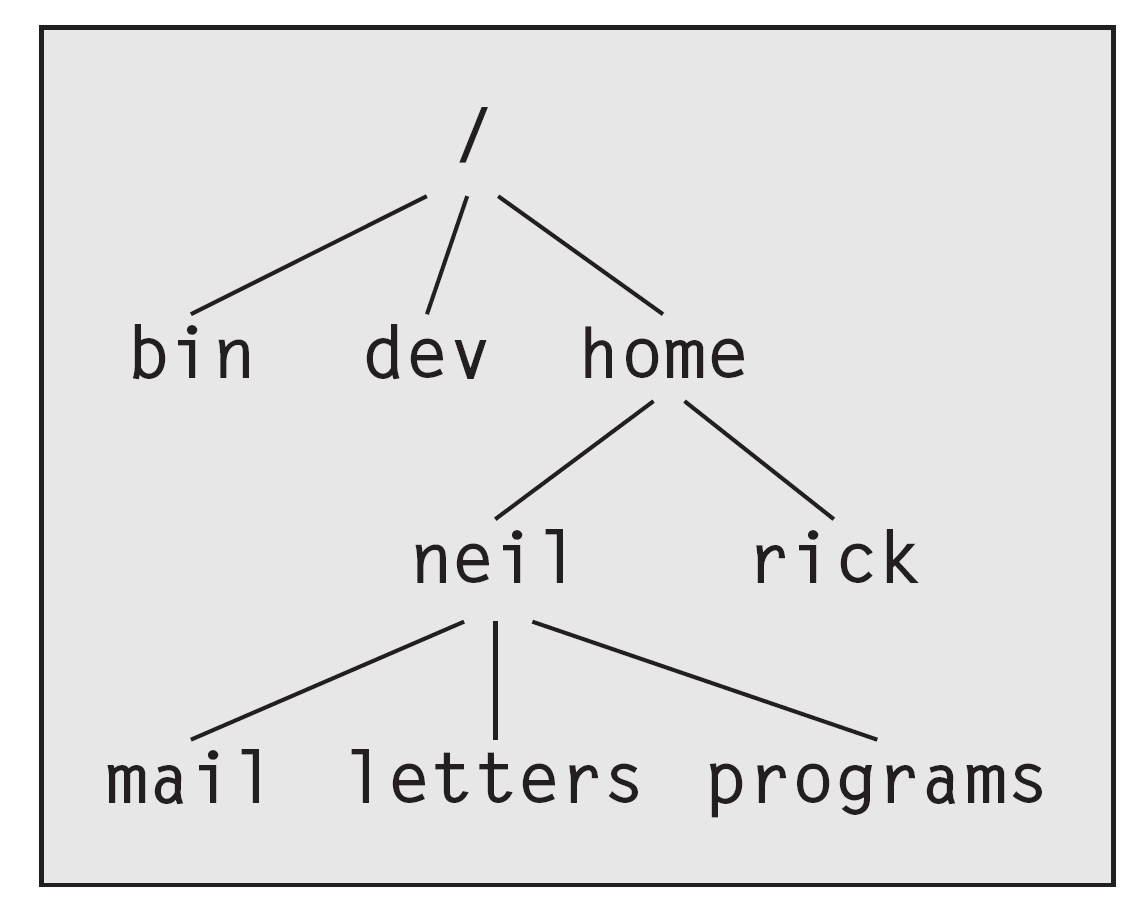
\includegraphics[width=1.0\textwidth]{../imgs/simple-directories.png}
%\begin{frame}{What is Profiling}
%\begin{itemize}
%\item Allows you to learn:
%\begin{itemize}
%\item where your program is spending its time
%\item what functions called what other functions
%\end{itemize}
%
%\item Can show you which pieces of your program are slower than you expected might be candidates for rewriting
%
%\item Are functions being called more or less often than expected? 
%
%\item This may help you spot bugs that had otherwise been unnoticed
%\end{itemize}
%\end{frame}
%
%%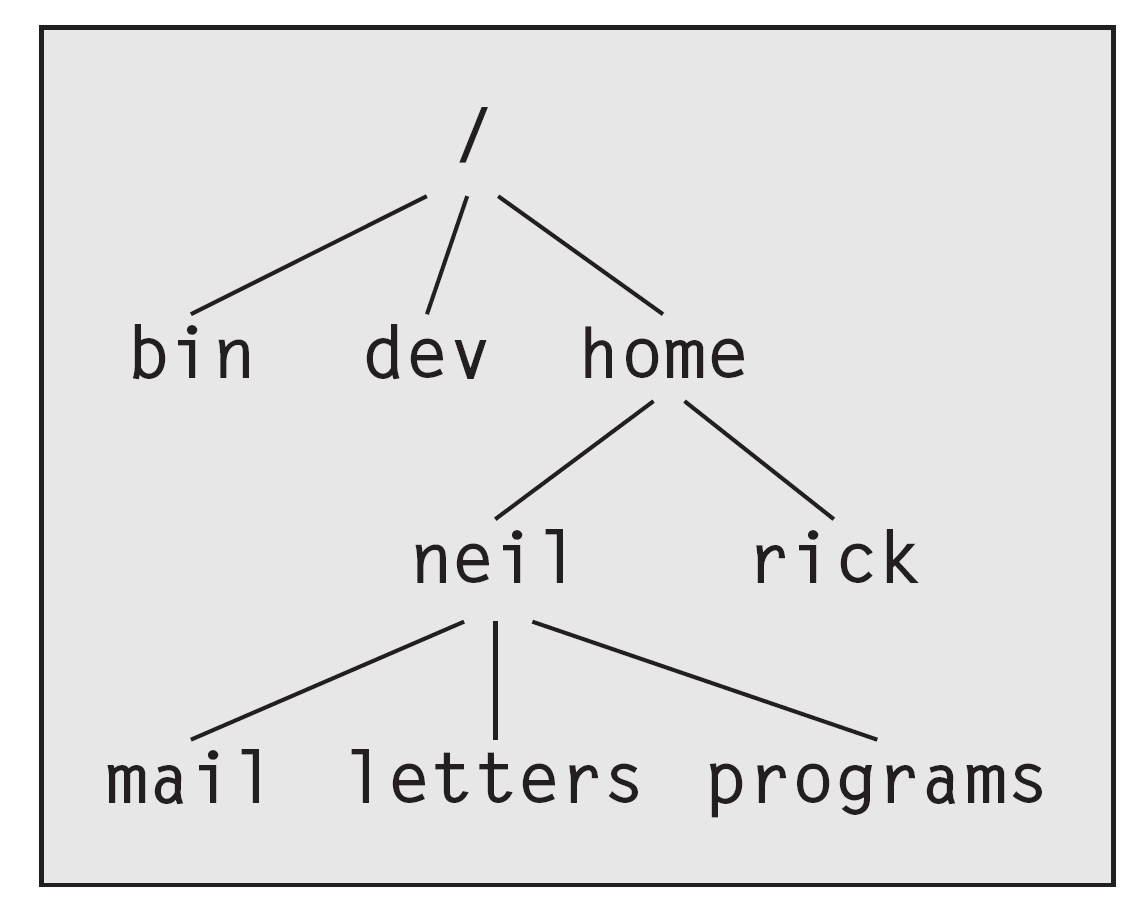
\includegraphics[width=1.0\textwidth]{../imgs/simple-directories.png}
%\begin{frame}{Profilier}
%\begin{itemize}
%\item It uses information collected during the actual execution of a program
%\item Can be used on programs that are too large or too complex to analyse by reading the source (or you are lazy.)
%\item How your program is run affects the information that shows up in the profile data
%\end{itemize}
%\end{frame}
%
%%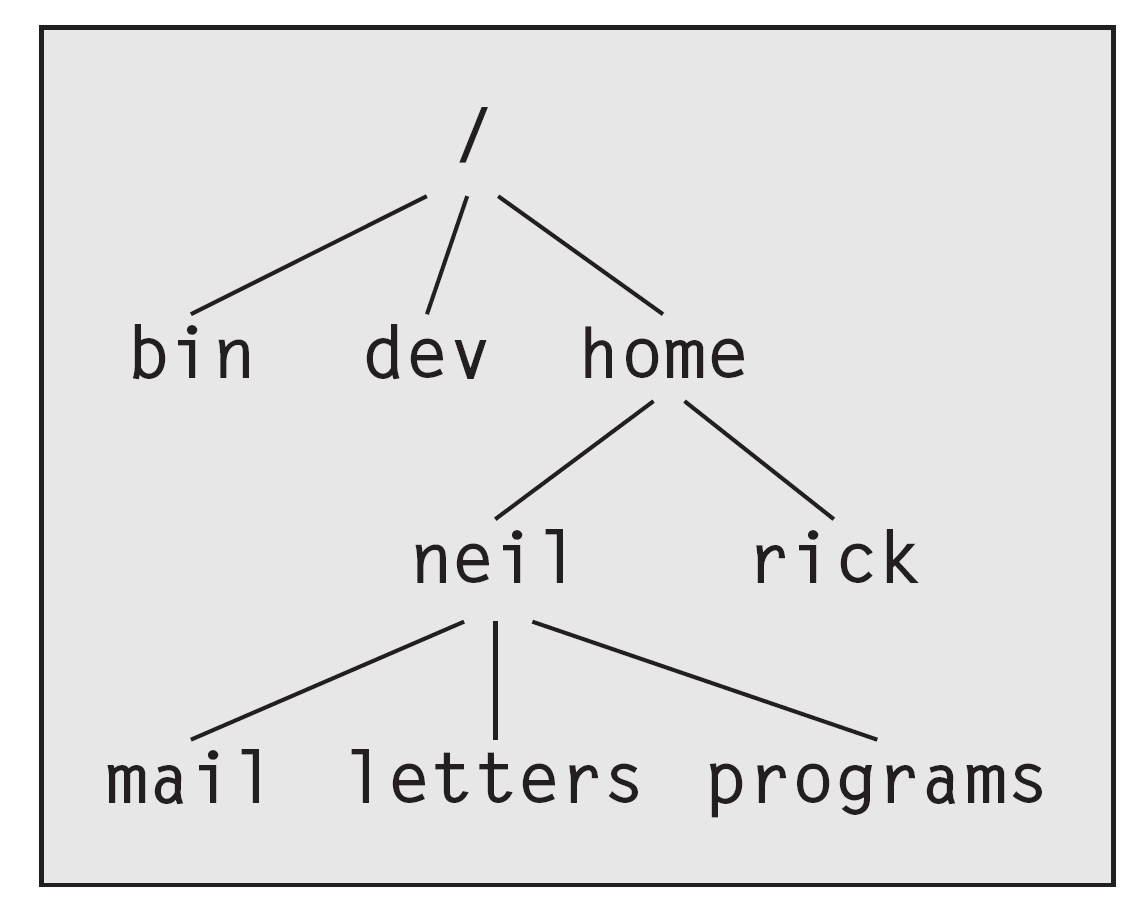
\includegraphics[width=1.0\textwidth]{../imgs/simple-directories.png}
%\begin{frame}{Profilier Steps}
%\begin{itemize}
%\item Compile and link your program with profiling enabled
%\item Often this is done by ``-pg'' option
%\item \$ gcc -Wall sampleCode.c -o sampleCode -pg
%\item Execute your program to generate a profile data file
%\item One important point to remember is that the program execution should happen in such a way that all the code blocks (or at least the ones you want to profile) get executed.
%\item \$ ./sampleCode
%\end{itemize}
%\end{frame}
%%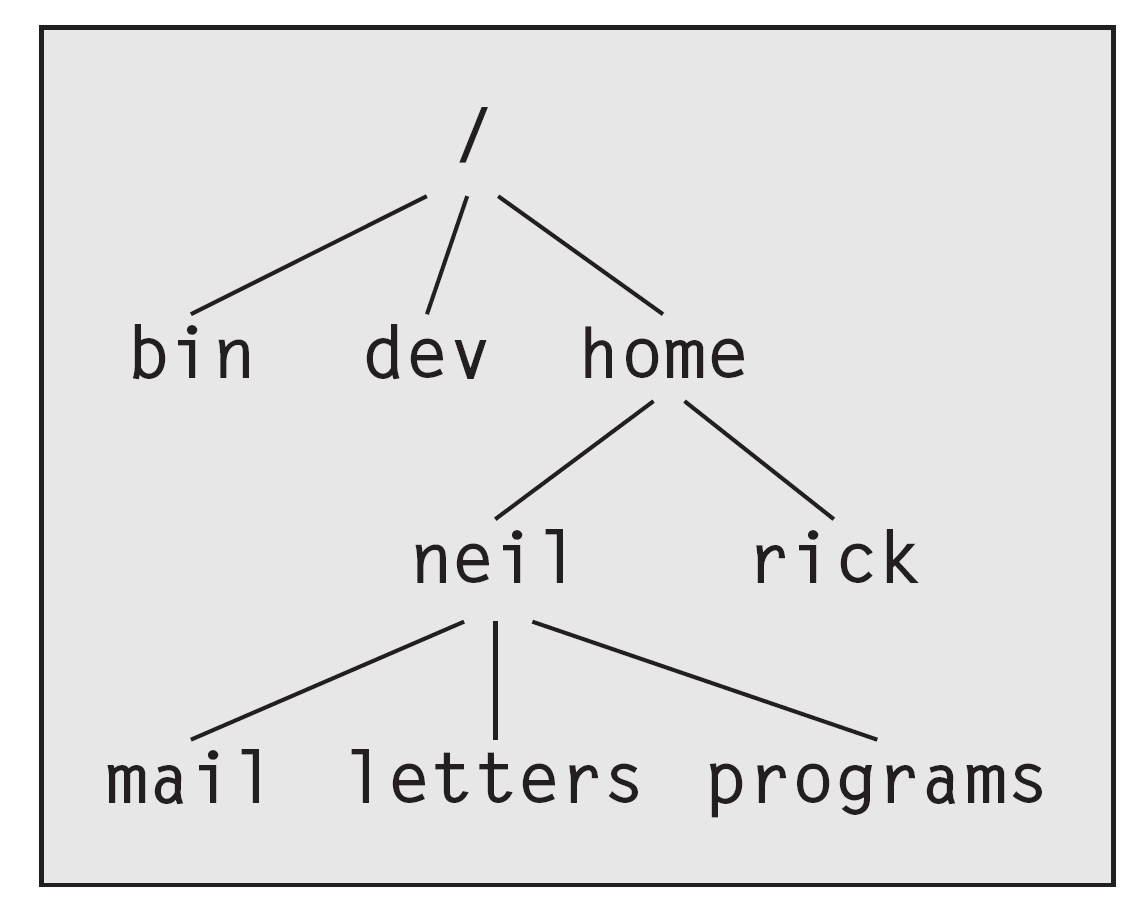
\includegraphics[width=1.0\textwidth]{../imgs/simple-directories.png}
%\begin{frame}{Profilier Steps Continued}
%\begin{itemize}
%\item Once the program is executed, it produces a file named gmon.out.
%\item This file contains the profiling data of the code blocks that were actually hit during the program execution. 
%\item It is not a regular text file and therefore cannot be read normally.
%\end{itemize}
%\end{frame}
%
%%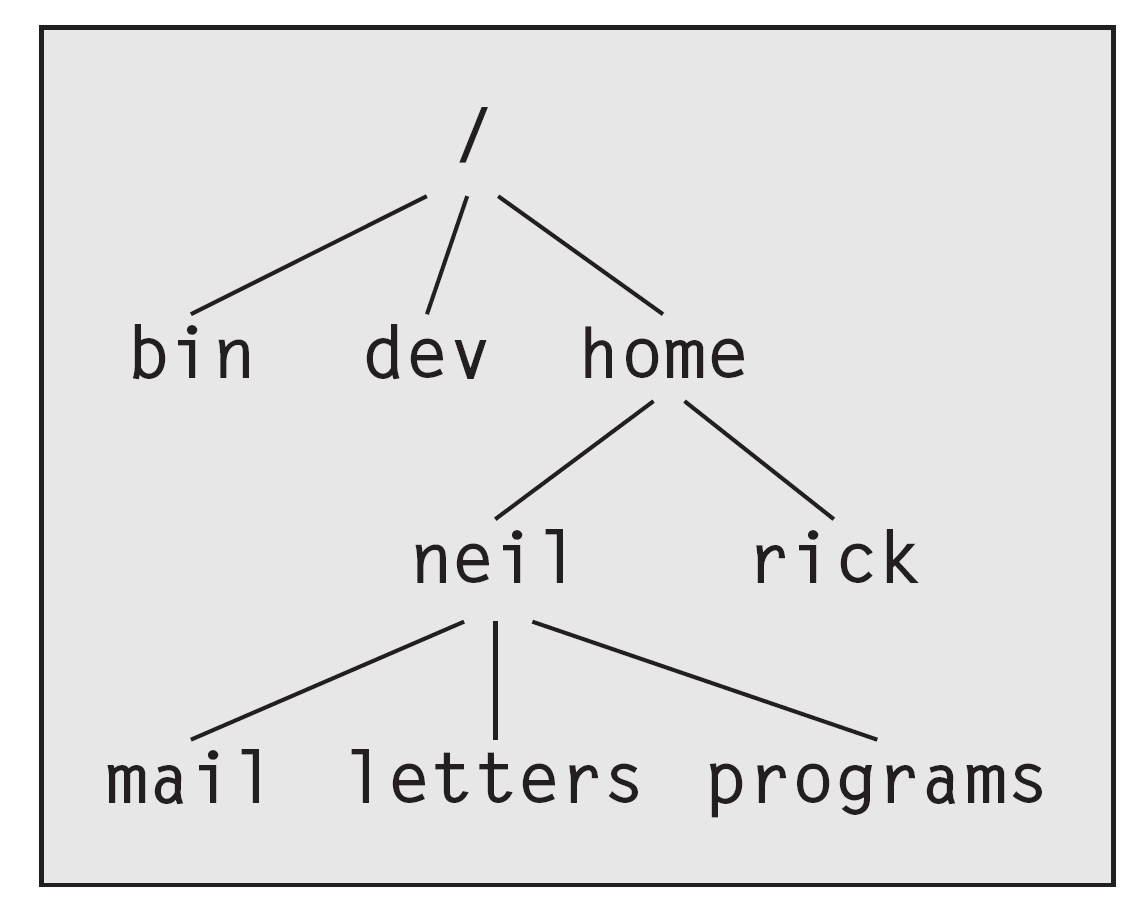
\includegraphics[width=1.0\textwidth]{../imgs/simple-directories.png}
%\begin{frame}{Profilier Steps Continued}
%\begin{itemize}
%\item Execute gprof
%\item Once the profiling data (gmon.out) is available, the gprof tool can be used to analyse and produce meaningful data from it.
%\item \$ gprof <command-line-options> <executable-file-name> <profiling-data-file-name> > <output-file>
%\item \$ gprof sampleCode gmon.out > prof\_output
%\end{itemize}
%\end{frame}
%
%%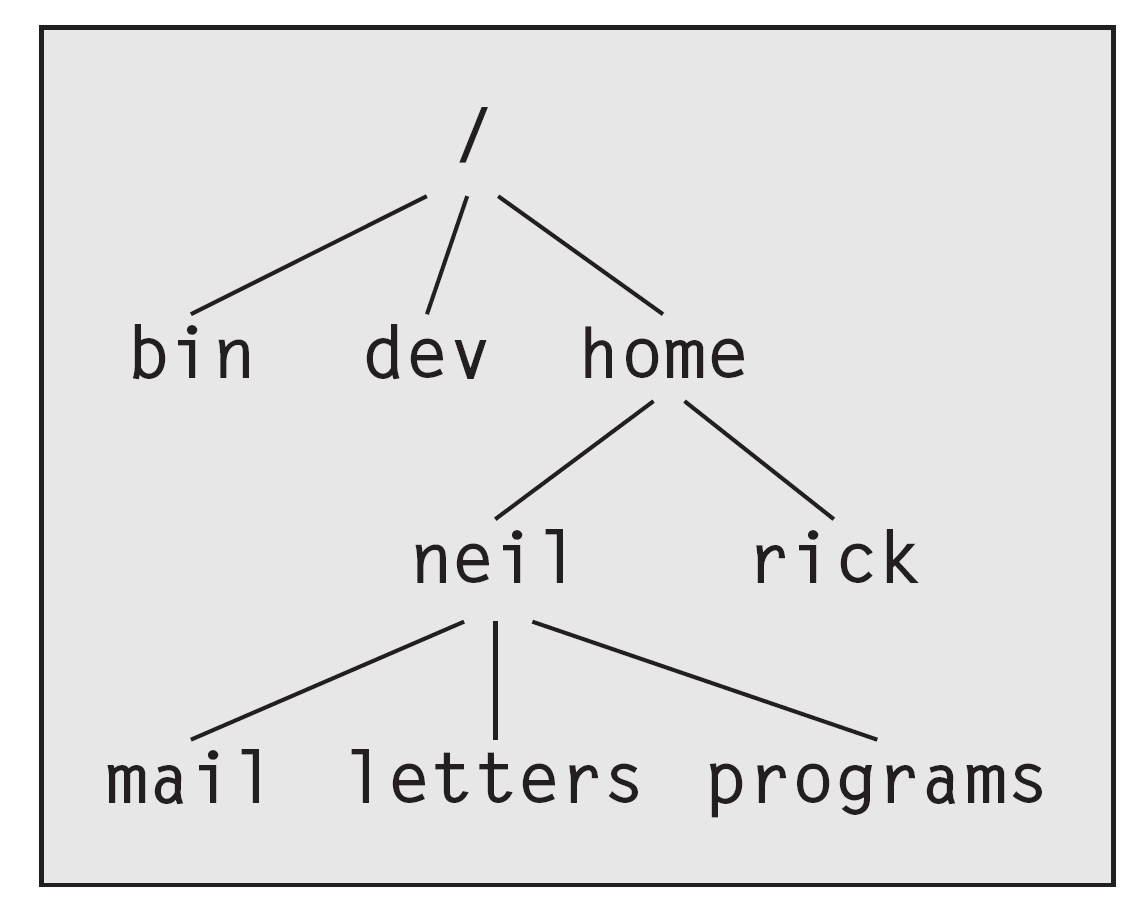
\includegraphics[width=1.0\textwidth]{../imgs/simple-directories.png}
%\begin{frame}{Example}
%\begin{columns}
%\column{0.50\textwidth}
%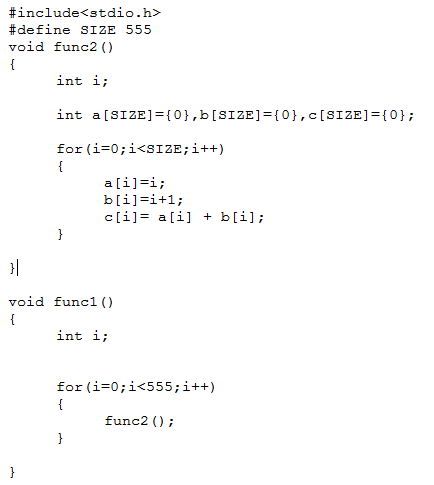
\includegraphics[width=1.0\textwidth]{../imgs/prof1.png}
%\column{0.50\textwidth}
%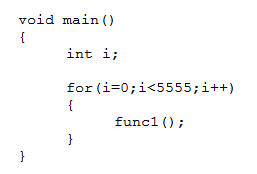
\includegraphics[width=1.0\textwidth]{../imgs/prof2.png}
%\end{columns}
%\end{frame}
%
%%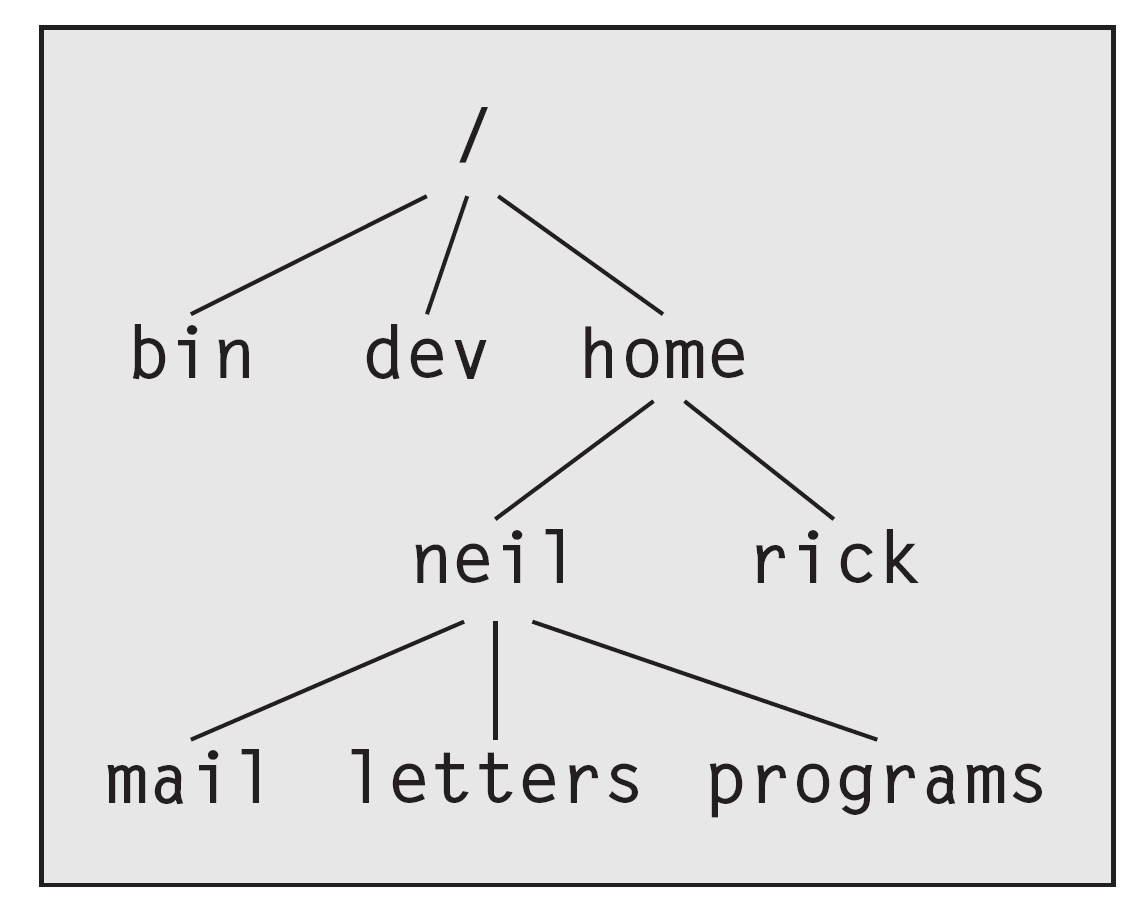
\includegraphics[width=1.0\textwidth]{../imgs/simple-directories.png}
%\begin{frame}{Flat Profile}
%\begin{itemize}
%\item time your program spent in each function
%\item how many times that function was called 
%\item information on which functions burn most of the cycles is clearly indicated here
%\end{itemize}
%\end{frame}
%
%%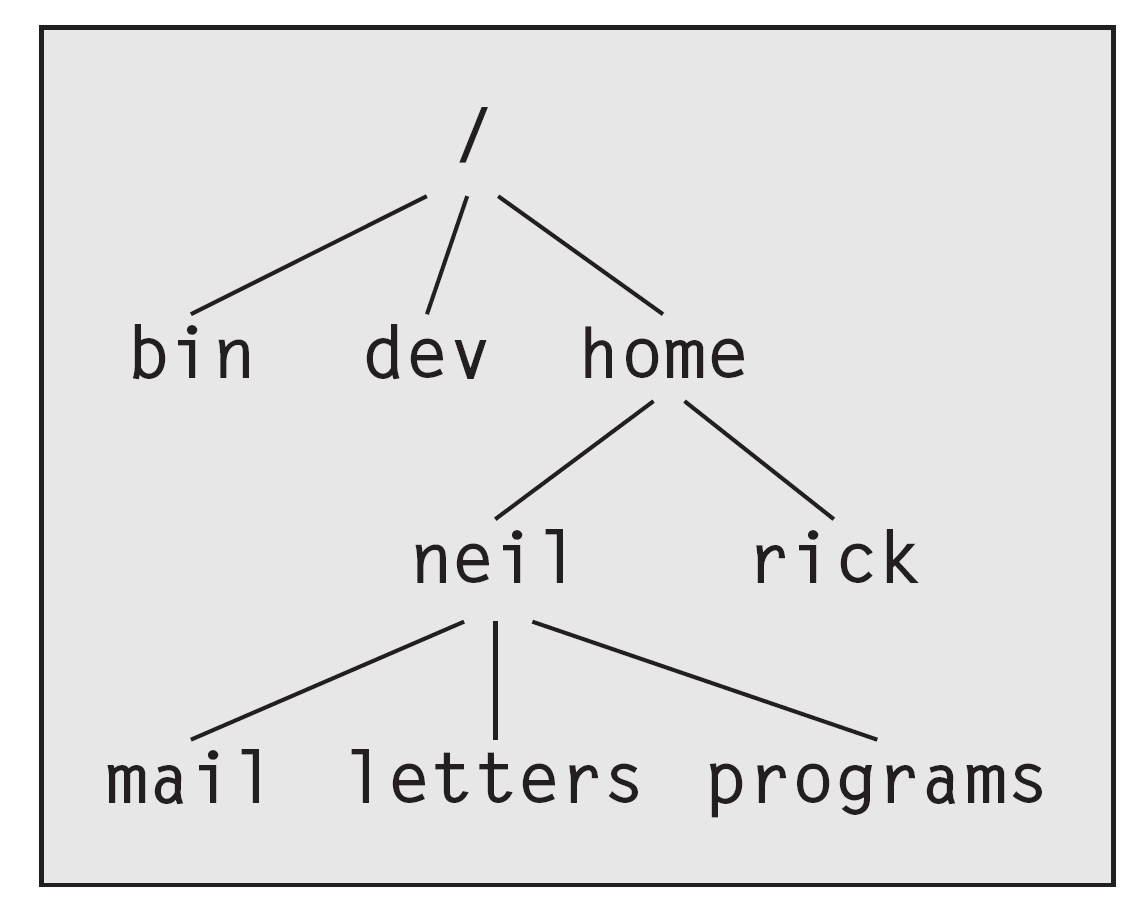
\includegraphics[width=1.0\textwidth]{../imgs/simple-directories.png}
%\begin{frame}{Flat Profile Results}
%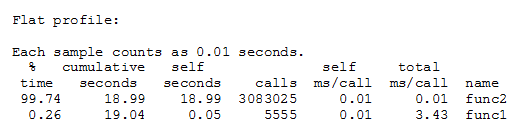
\includegraphics[width=1.0\textwidth]{../imgs/prof3.png}
%\begin{itemize}
%\item \textbf{\% time} percentage of the total execution time program spent in this function \\
%all functions combined should add up to 100\%!
%\item \textbf{cumulative seconds}
%This is the cumulative total number of seconds  spent executing this function plus the time spent in all the functions above this one in this table
%\item \textbf{self seconds}
%number of seconds accounted for by this function alone  
%\item flat profile listing is sorted first by this number
%\end{itemize}
%\end{frame}
%
%%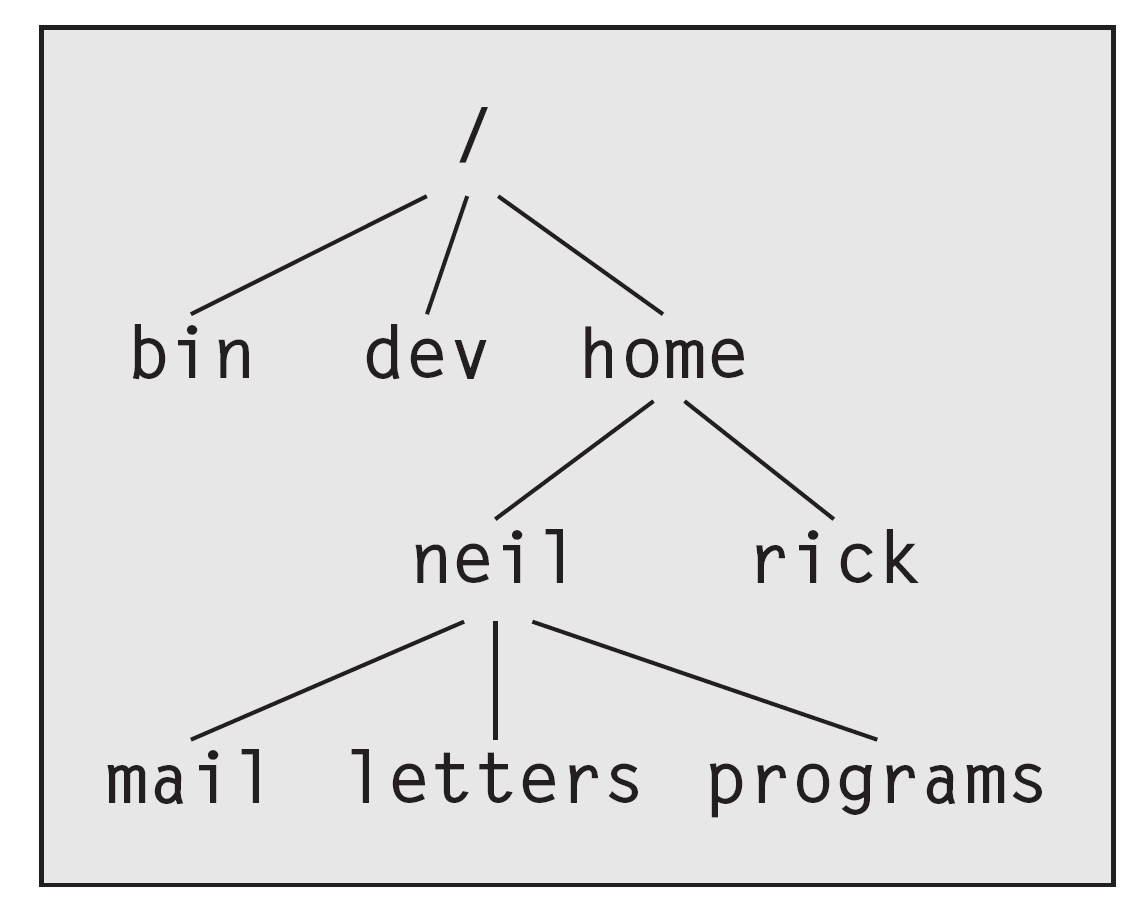
\includegraphics[width=1.0\textwidth]{../imgs/simple-directories.png}
%\begin{frame}{}
%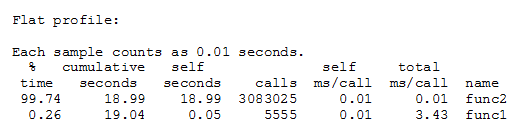
\includegraphics[width=1.0\textwidth]{../imgs/prof3.png}
%\begin{itemize}
%\item \textbf{calls}
%total number of times the function was called 
%if the function was never called, or the number of times it was called cannot be determined (probably because the function was not compiled with profiling enabled), the calls field is blank
%
%\item \textbf{self ms/call}
%represents the average number of milliseconds spent in this function per call
%if this function is not profiled this field is blank 
%
%\item \textbf{total ms/call}
%represents the average number of milliseconds spent in this function and its descendants per call
%if this function is not profiled this field is blank
%\end{itemize}
%\end{frame}
%
%%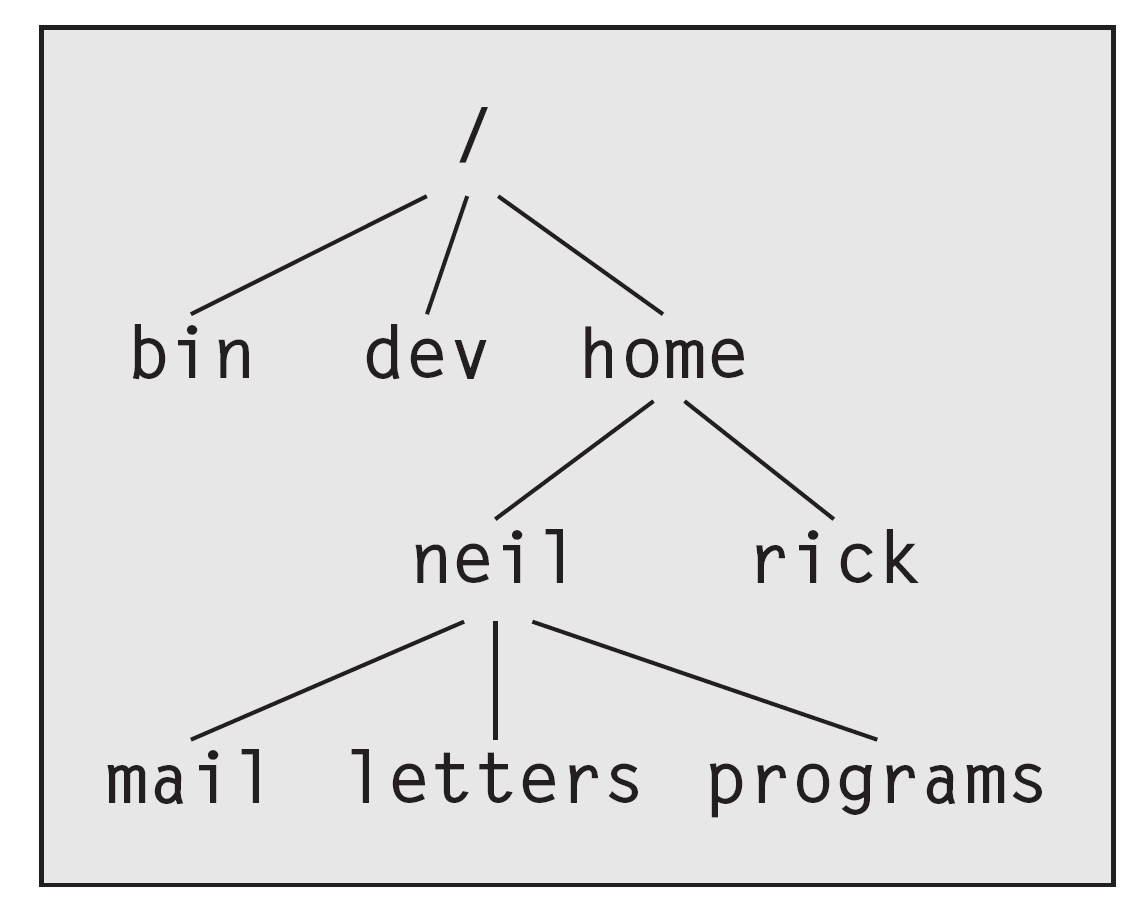
\includegraphics[width=1.0\textwidth]{../imgs/simple-directories.png}
%\begin{frame}{Call Graph}
%\begin{itemize}
%\item shows, for each function: 
%\item which functions called it, 
%\item which other functions it called,  
%\item how many times it was called. 
%
%\item an estimate of how much time was spent in the subroutines of each function 
%
%\item suggests places where you might try to eliminate function calls that use a lot of time.
%\end{itemize}
%\end{frame}
%
%\begin{frame}{Call Graph}
%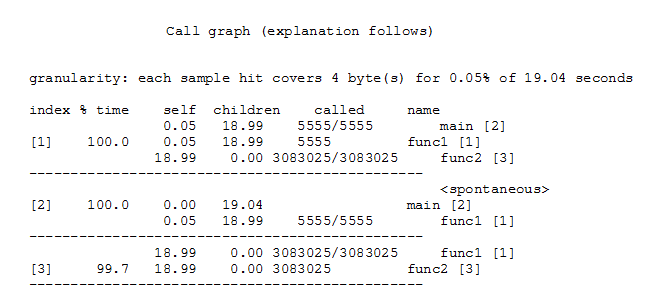
\includegraphics[width=1.0\textwidth]{../imgs/prof4.png}
%\end{frame}
%
%\begin{frame}{Limitations}
%\begin{itemize}

%\item profiling is taken at fixed intervals of run time (so count may be different between runs!)
%\item There are numerous events that may throw off your analysis from actual experiments:
%\begin{itemize}
%\item Varying processor speeds
%\item Varying memory systems (Caches, L1, L2, Main)
%\item Disk speeds \& Network Traffic(I/O operations)
%\item Software instrumentations (what type of optimizations did you uses?)
%\item Computer load during runs
%\end{itemize}
%\item These are beyond the scope fo this class.
%\item Be aware that gprof may give anomalous results (and be ready for them).
%\item Like Newtonian Physics, gprof can be a good approximation.
%\end{itemize}
%\end{frame}

\section{Gnuplot}
\subsection{}

%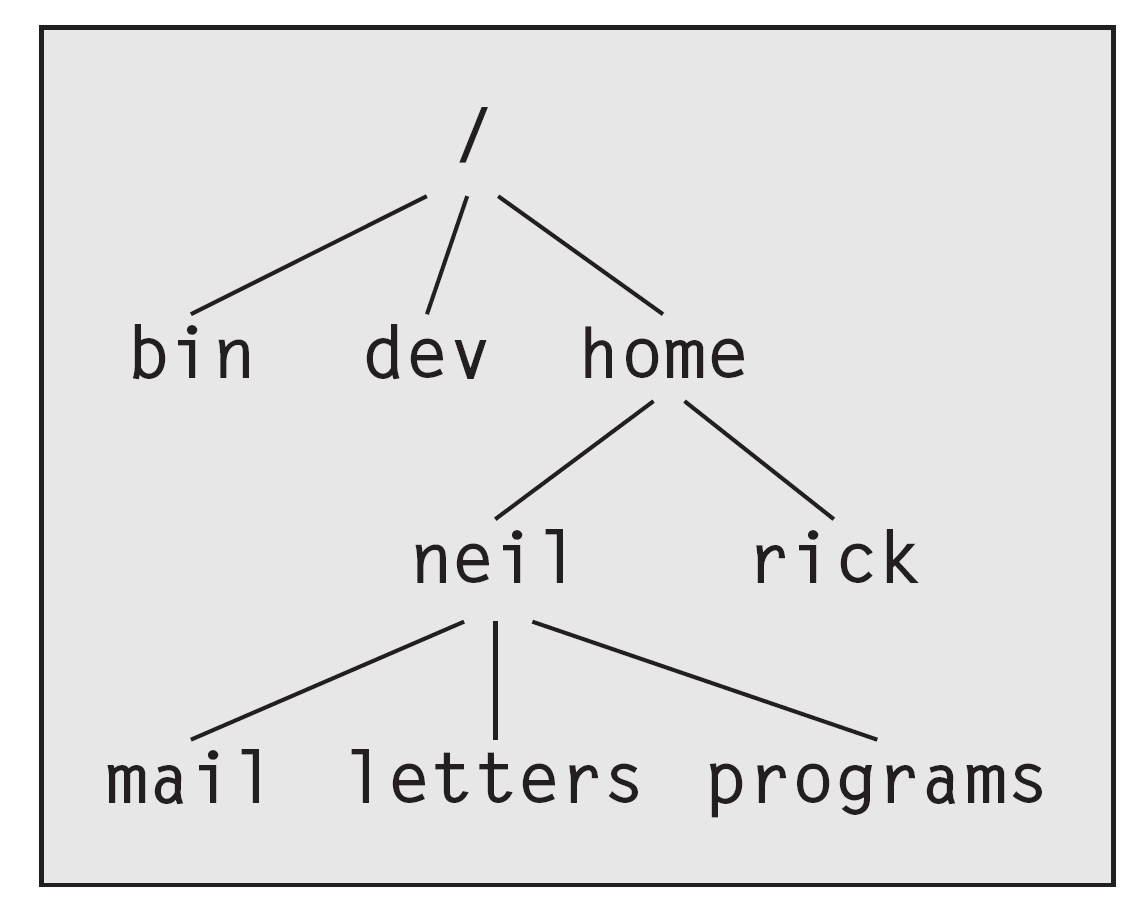
\includegraphics[width=1.0\textwidth]{../imgs/simple-directories.png}
\begin{frame}{Crash Course}
\begin{itemize}
\item gnuplot makes graphs
\item type ``gnuplot'' at your terminal 
\item type ``plot sin(x) with line''
\item type ``plot sin(x) with point''

\item Type ``set terminal postscript color''
\item Type ``set output ``nameofplot.ps'' ''
\item Type ``replot'' or ``rep''
\end{itemize}
\end{frame}

%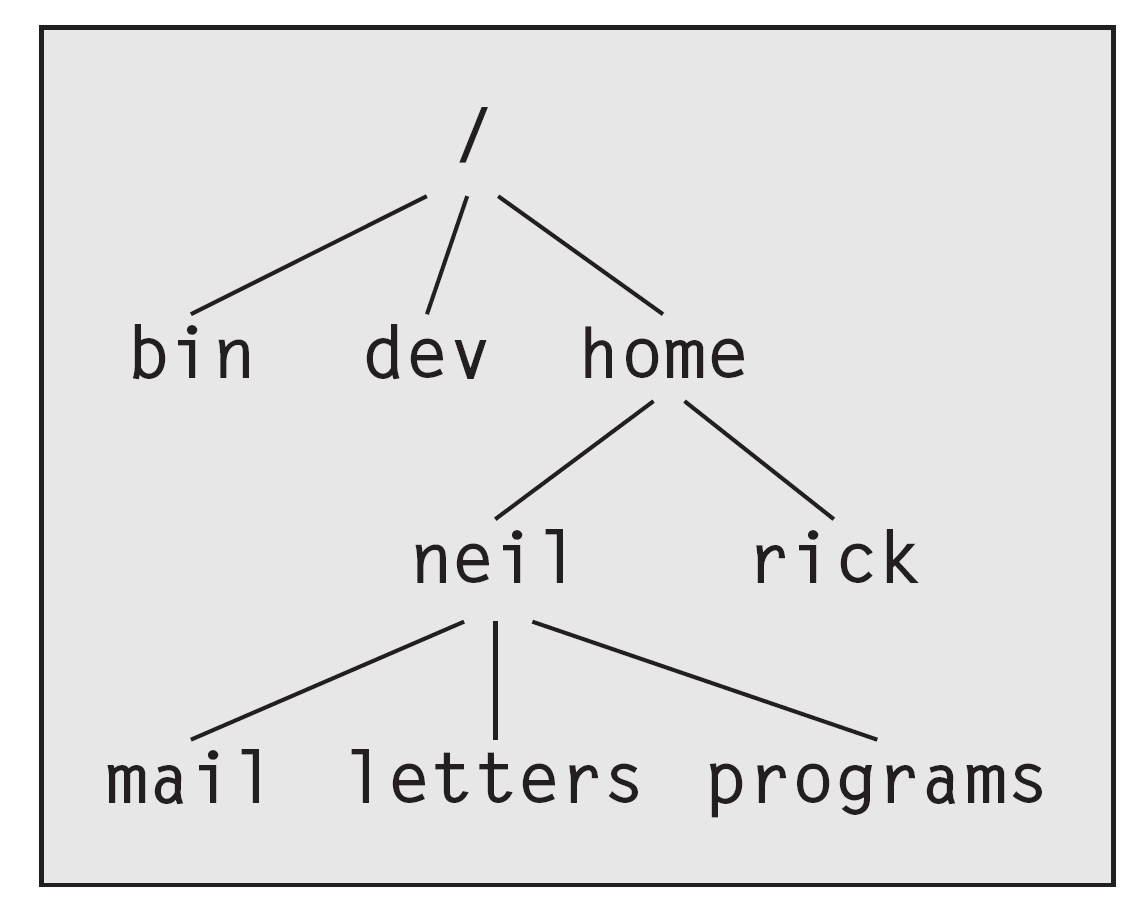
\includegraphics[width=1.0\textwidth]{../imgs/simple-directories.png}
\begin{frame}{Continued}
\begin{itemize}
\item Type ``set title ``plotname'' ''
\item Type ``set ylabel ``ylabel'' ''                                    
\item Type ``set xlabel ``xlabel'' ''

\item to covert to something readable (like pdf).  On the command line do:\\
\$ ps2pdf nameofplot.ps
\item Then you should have nameofplot.pdf \\
\$ evince nameofplot.pdf
\end{itemize}
\end{frame}

\begin{frame}[fragile]{Huge Time Saver!}
\begin{itemize}
\item The commands to gnuplot can be saved to a file and then automatically used:
\item simple.plot:\\
\begin{lstlisting}
set terminal postscript color
set output "simple.ps"
set ylabel "time (seconds)"
set xlabel "size"

...
\end{lstlisting}
\item \$ gnuplot simple.plot
\item \$ ps2pdf simple.ps
\item \$ evince simple.pdf
\item Will display the graph.
\item This is especially useful if you put it in a makefile!
\begin{lstlisting}
plot:
        gnuplot simple.plot
        ps2pdf simple.ps
        evince simple.pdf
\end{lstlisting}
\item Now ''\$ make plot'' generates the graph and displays it!
\end{itemize}
\end{frame}

\section{Perf}
\subsection{}

\begin{frame}{Perf}
\begin{itemize}
\item Tool to find what part of the code is running slow.
\item Steps:
\begin{enumerate}
\item compile with debug flags! (-g)
\item run: \\
%\$ sudo perf record --call-graph dwarf <your-programs-name>
\$ sudo perf record <your-programs-name>
\item view the report:\\
\$ sudo perf report
\end{enumerate}
\item Now you should see what functions are taking up all the time!
\end{itemize}
\includegraphics[width=1.0\textwidth]{../imgs/perf.png}
\end{frame}

\section{Timing}
\subsection{}

%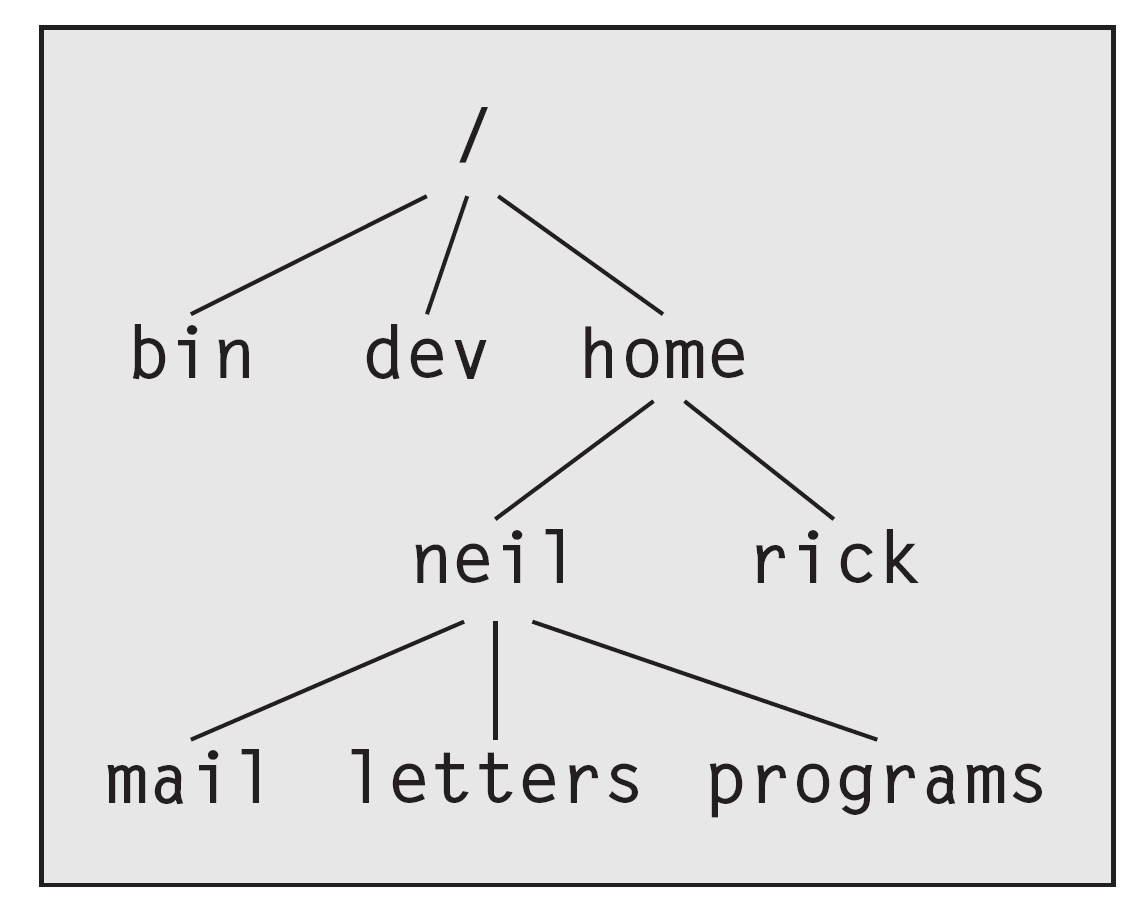
\includegraphics[width=1.0\textwidth]{../imgs/simple-directories.png}
\begin{frame}{Emperical Measurement}
\begin{itemize}
\item While Analytical measurement of performance is important sometimes an emperical approach is most useful.
\item The naive way to take timings:
\begin{enumerate}
\item Record time as start
\item Run section of code you wish to time
\item Record time as end
\item You answer is (end - start).
\end{enumerate}
\item While there are numerous issues with this approach, it will give sufficient approximate timings for this class.
\end{itemize}
\end{frame}

%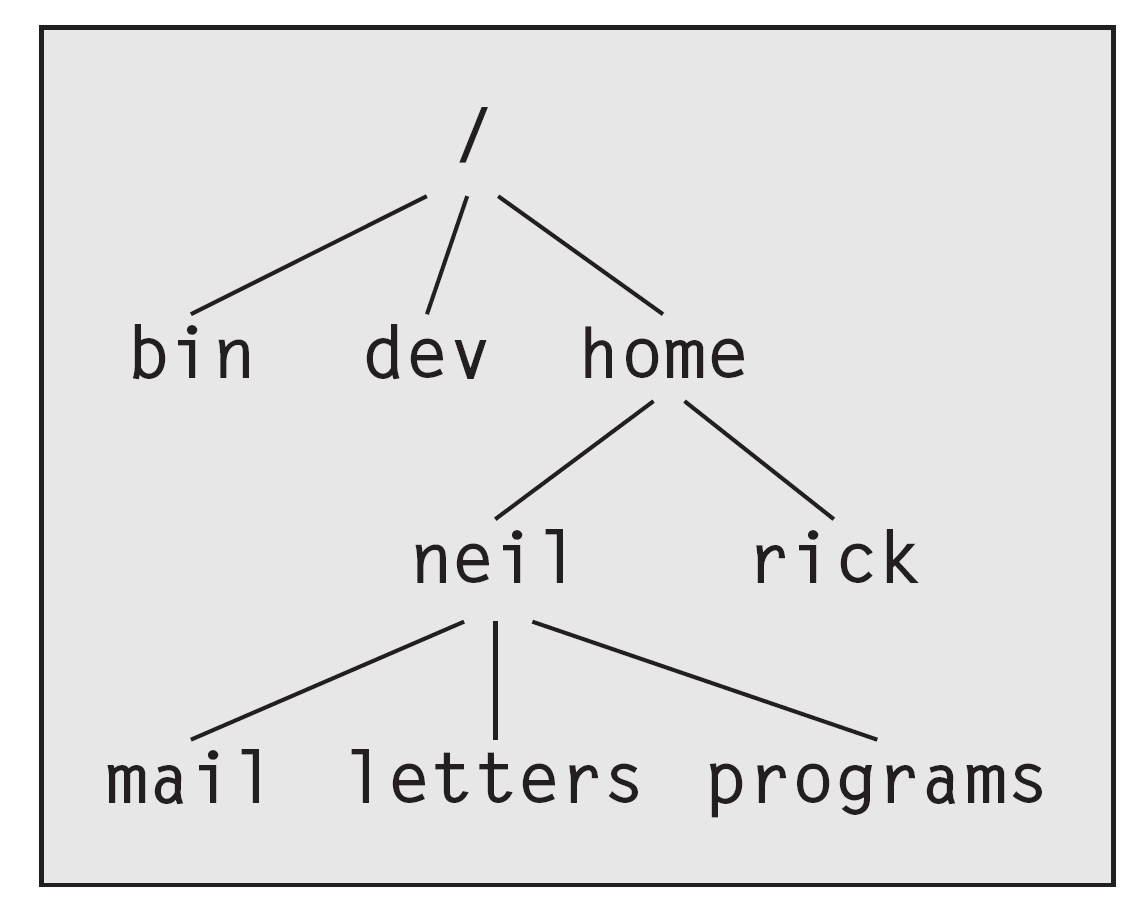
\includegraphics[width=1.0\textwidth]{../imgs/simple-directories.png}
\begin{frame}[fragile]{}
\begin{lstlisting}
#include <iostream> // To print
#include <time.h> // Required for taking timings

int main(int argc, char *argv[]) { // Standard main heading.
    /* clock_t is the data type for storing timing information.
     * We must make two variables, one for the start and the other to capture
     * the difference.
     */
    clock_t start, diff;

    // timeAmount is used to print out the time in seconds.
    double timeAmount;

    // We want to run our algorithm over varying sizes.
    for (int i = 1000; i < 1000000; i += 1000) {
        // Capture the start clock
        start = clock();

        // This is were your algorithm should be called.
        functionCallToYouAlgorithm(i);

        // Capture the clock and subtract the start to get the total time elapsed.
        diff = clock() - start;

        // Convert clock_t into seconds as a floating point number.
        timeAmount = diff * 1.0 / CLOCKS_PER_SEC;

        // Print out first the size (i) and then the elapsed time.
        std::cout << i << " " << timeAmount << "\n";

        // We flush to ensure the timings is printed out.
        std::cout << std::flush;
    }
    return 0;
}

\end{lstlisting}
\end{frame}

%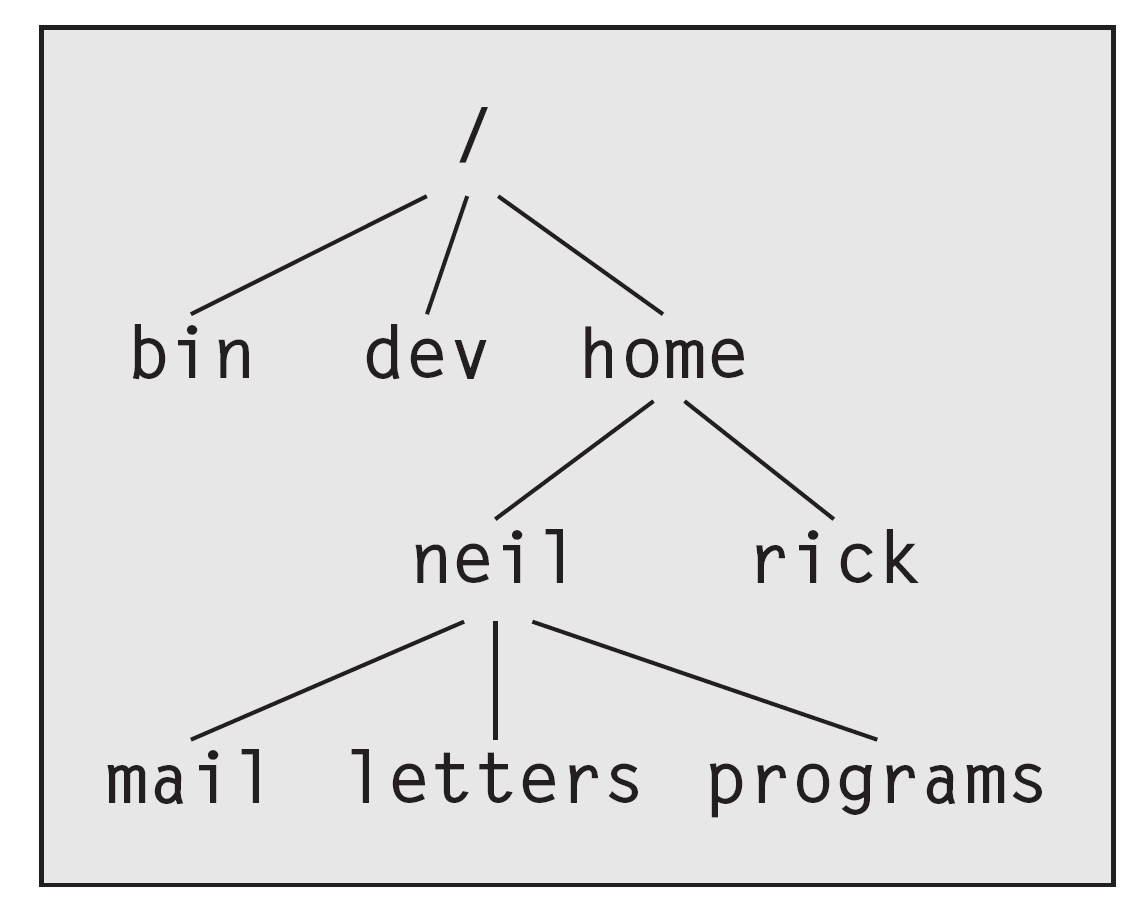
\includegraphics[width=1.0\textwidth]{../imgs/simple-directories.png}
\begin{frame}[fragile]{Example Output}
\begin{lstlisting}
1000 4e-06
2000 8e-06
3000 1.2e-05
4000 2.5e-05
5000 2.9e-05
6000 2.4e-05
7000 3.5e-05
8000 2.9e-05
9000 3.2e-05
10000 3.5e-05
11000 3.9e-05
12000 4.2e-05
13000 4.5e-05
14000 5.2e-05
15000 5.6e-05
16000 6e-05
17000 6.5e-05
18000 6.8e-05
19000 7e-05
20000 7.6e-05
\end{lstlisting}
\begin{itemize}
\item First is the size (1000) and second is the number of seconds (pretty small.)
\end{itemize}
\end{frame}

%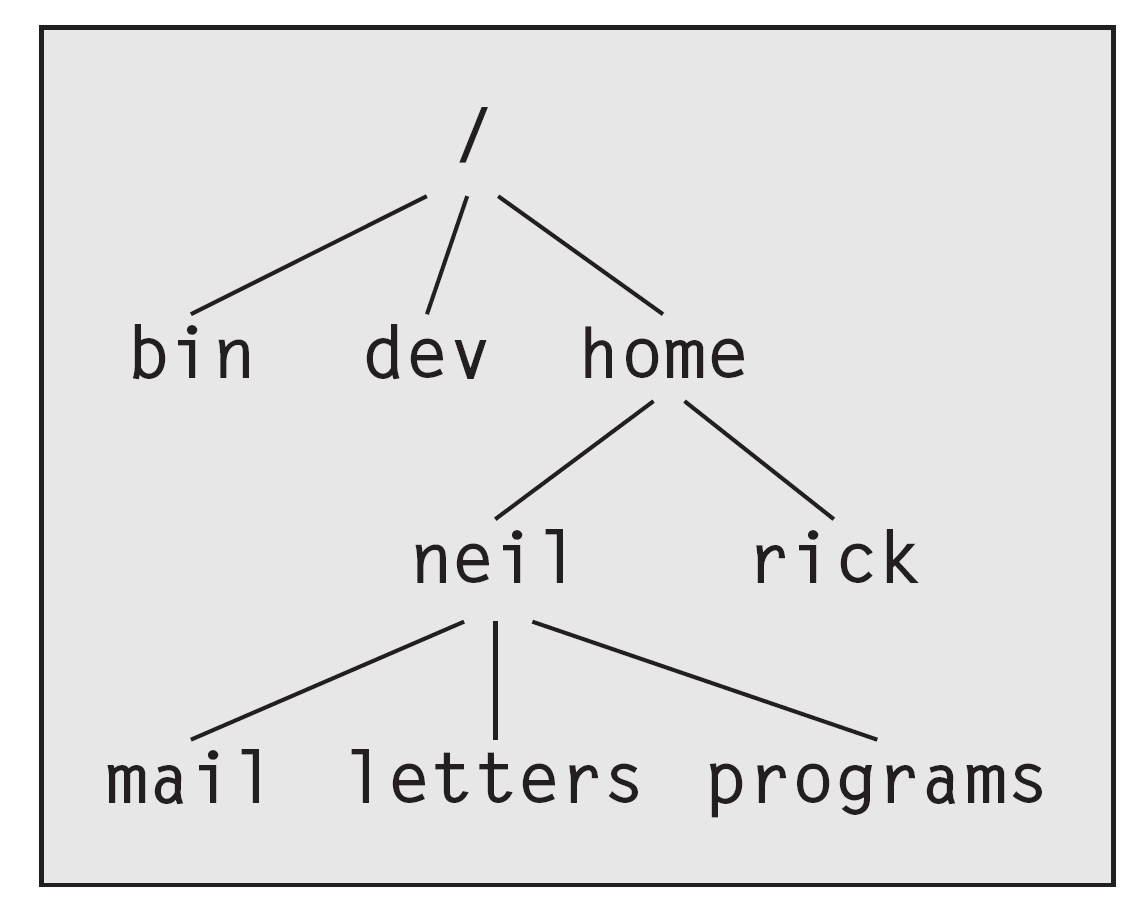
\includegraphics[width=1.0\textwidth]{../imgs/simple-directories.png}
\begin{frame}{Plotting}
\begin{columns}
\column{0.60\textwidth}
\begin{itemize}
\item First lets us assume we have the full listing in a file named 'single-timings'
\item With gnuplot we can simply graph the timings: \\
plot [:][:] ``single-timings'' using 1:2 with line
\end{itemize}
\column{0.40\textwidth}
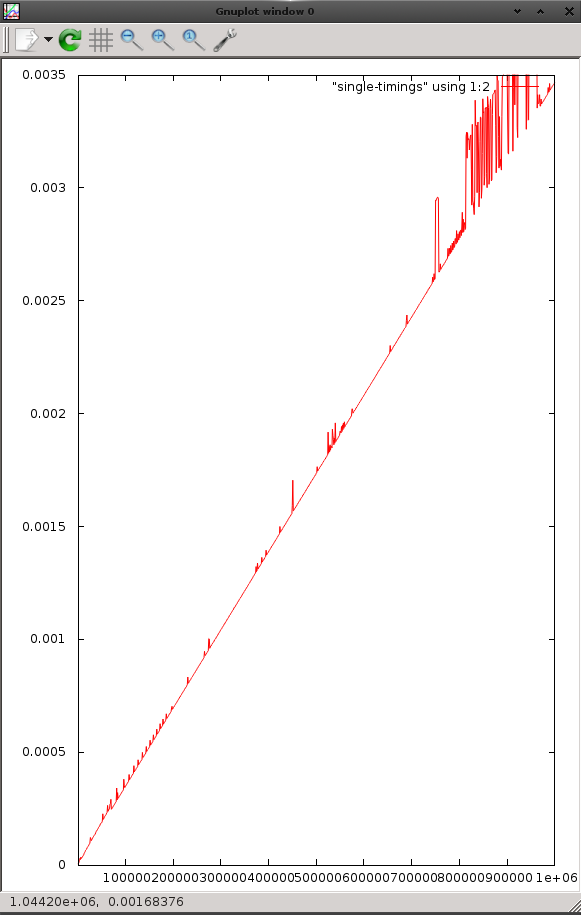
\includegraphics[width=1.0\textwidth]{../imgs/timings1.png}
\end{columns}
\end{frame}

%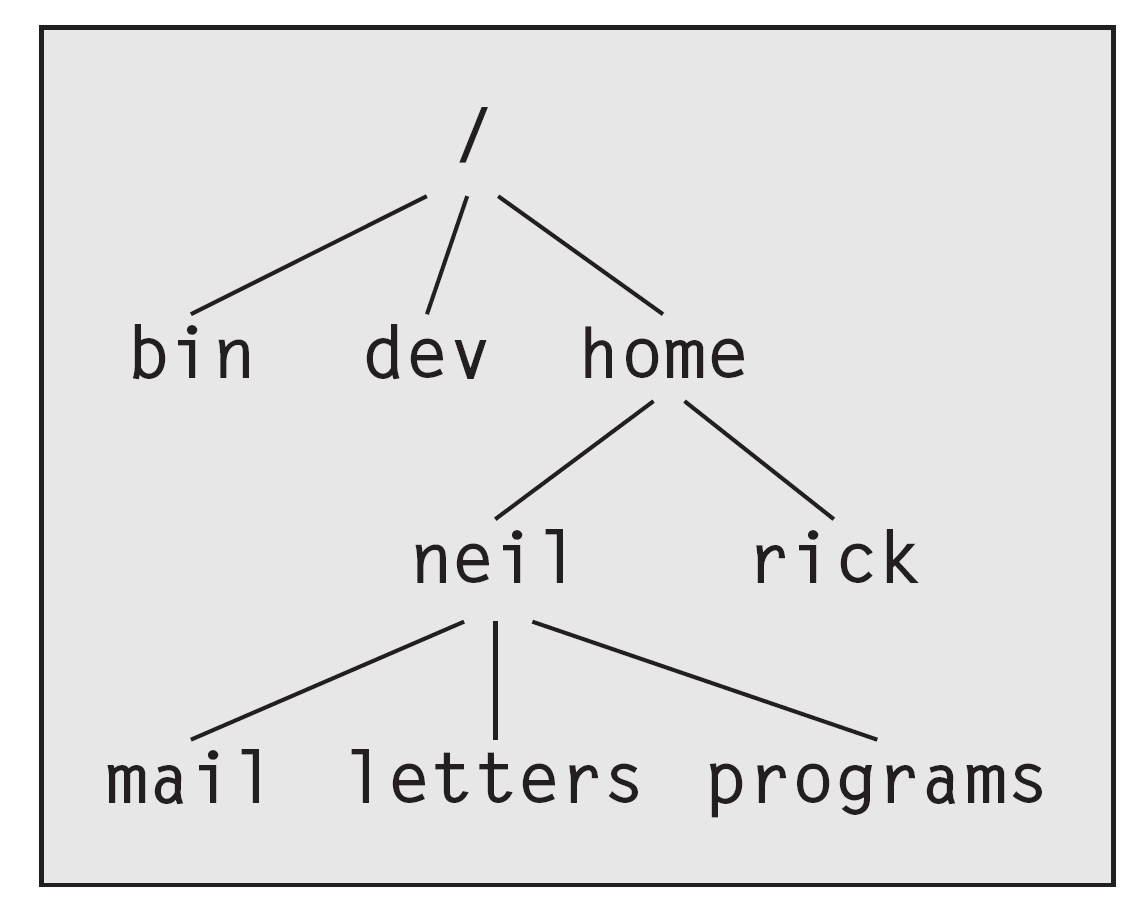
\includegraphics[width=1.0\textwidth]{../imgs/simple-directories.png}
\begin{frame}{Multiple Data Collections}
\begin{columns}
\column{0.50\textwidth}
\begin{itemize}
\item In addition to 'single-timings' let us assume we have another file (in the same format) named 'squared-enhanced-timings'
\item With gnuplot we can graph both timings: \\
plot [:][:] ``single-timings'' using 1:2 with line, ``squared-enhanced-timings'' using 1:2 with line
\item {\tiny You can append more and more data files in this manner.}
\end{itemize}
\column{0.50\textwidth}
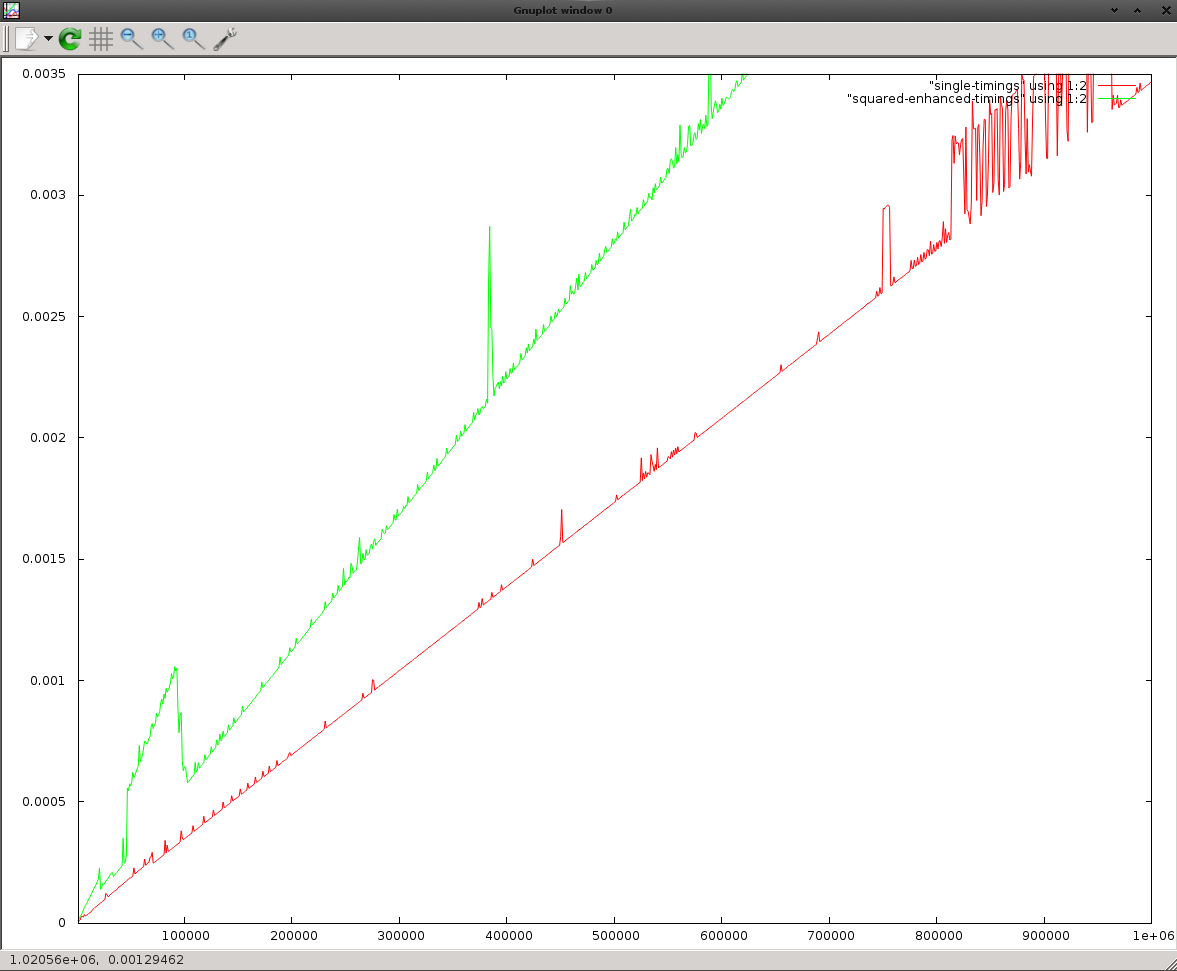
\includegraphics[width=1.0\textwidth]{../imgs/timings2.png}
\end{columns}
\end{frame}

\section{Tips \& Gotchas}
\subsection{}

%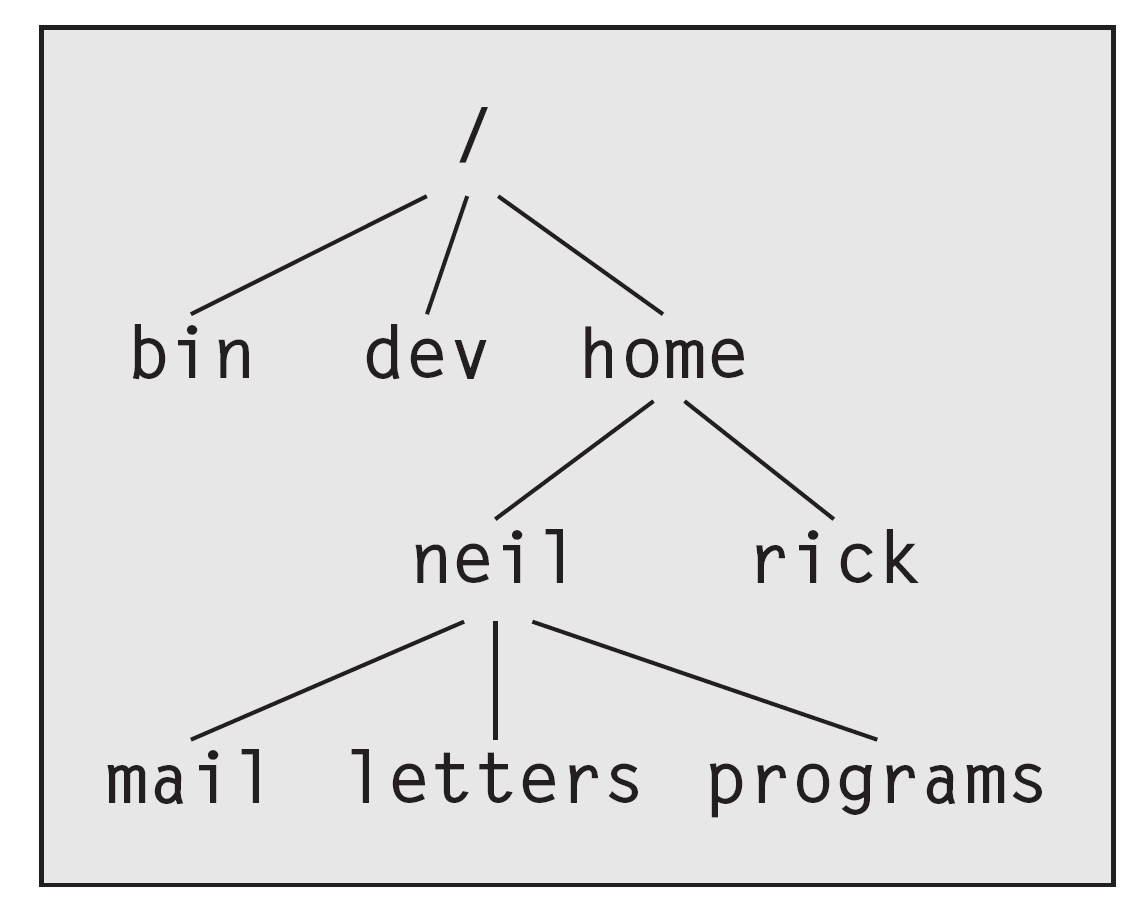
\includegraphics[width=1.0\textwidth]{../imgs/simple-directories.png}
\begin{frame}{Summary}
\begin{itemize}
\item Hopefully you can see from today that we can:
\begin{itemize}
\item Analyze algorithm analytically to predict performance.
\item Profile code to find what piece of code is the bottleneck.
\item Get \& plot timings to see actual performance.
\end{itemize}
\item Performance Analysis could take the whole class time.
\item We stick with the basics for this class.
\item I do want to alert you to a couple of things that will help!
\end{itemize}
\end{frame}

\begin{frame}{Gotcha 1}
\begin{columns}
\column{0.50\textwidth}
\begin{itemize}
\item You plot the data of two algorithms, but you can see only one!
\item <2-> Check your data and axis, usually it is because it is too small to see.
\item <3-> {\tiny plot [:][:] "single-timings" using 1:2 with line, "squared-timings" using 1:2 with line -> \\
plot [:][:2] "single-timings" using 1:2 with line, "squared-timings" using 1:2 with line }

\end{itemize}
\column{0.50\textwidth}
\only<1-1> {
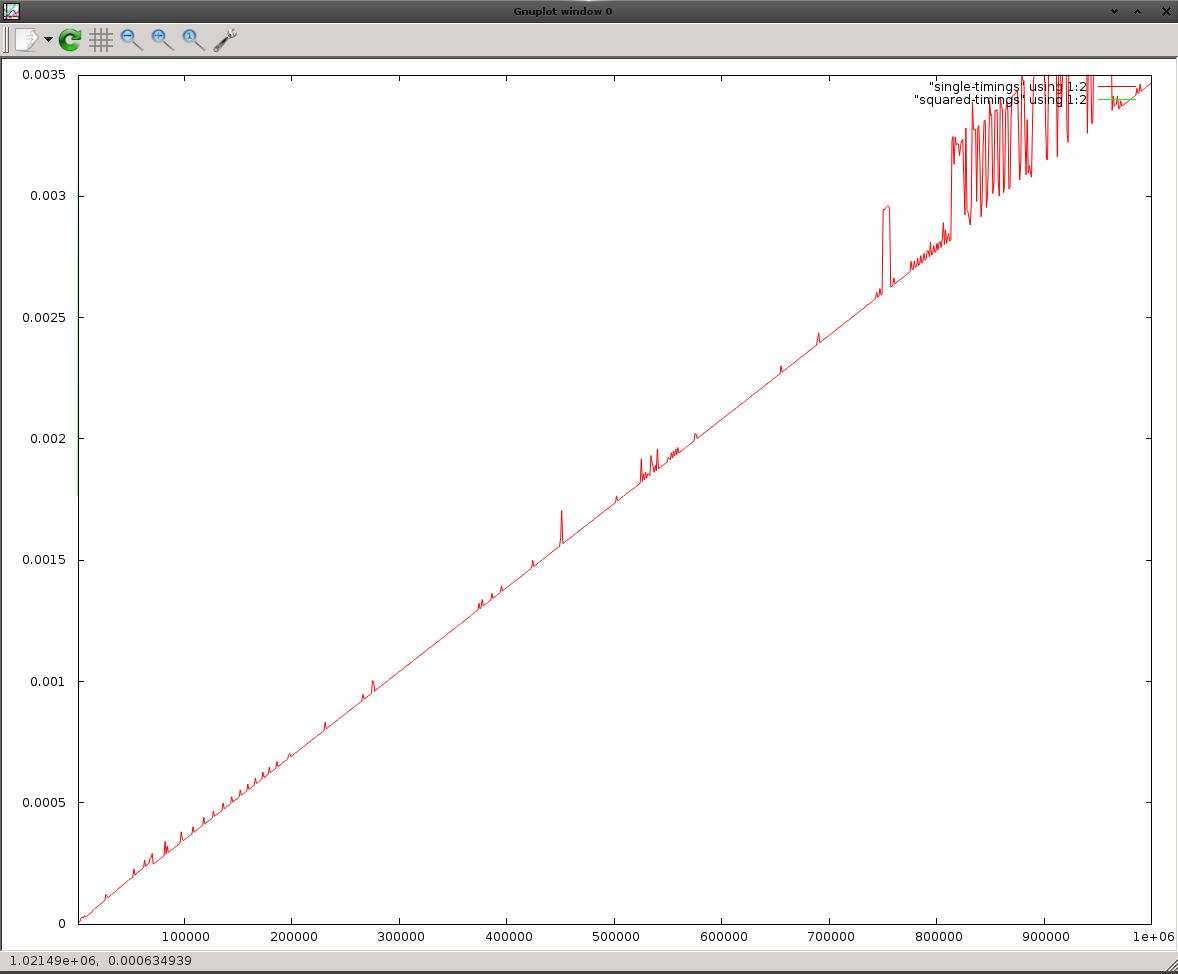
\includegraphics[width=1.0\textwidth]{../imgs/timing-gotcha1.png}
}
\only<2-> {
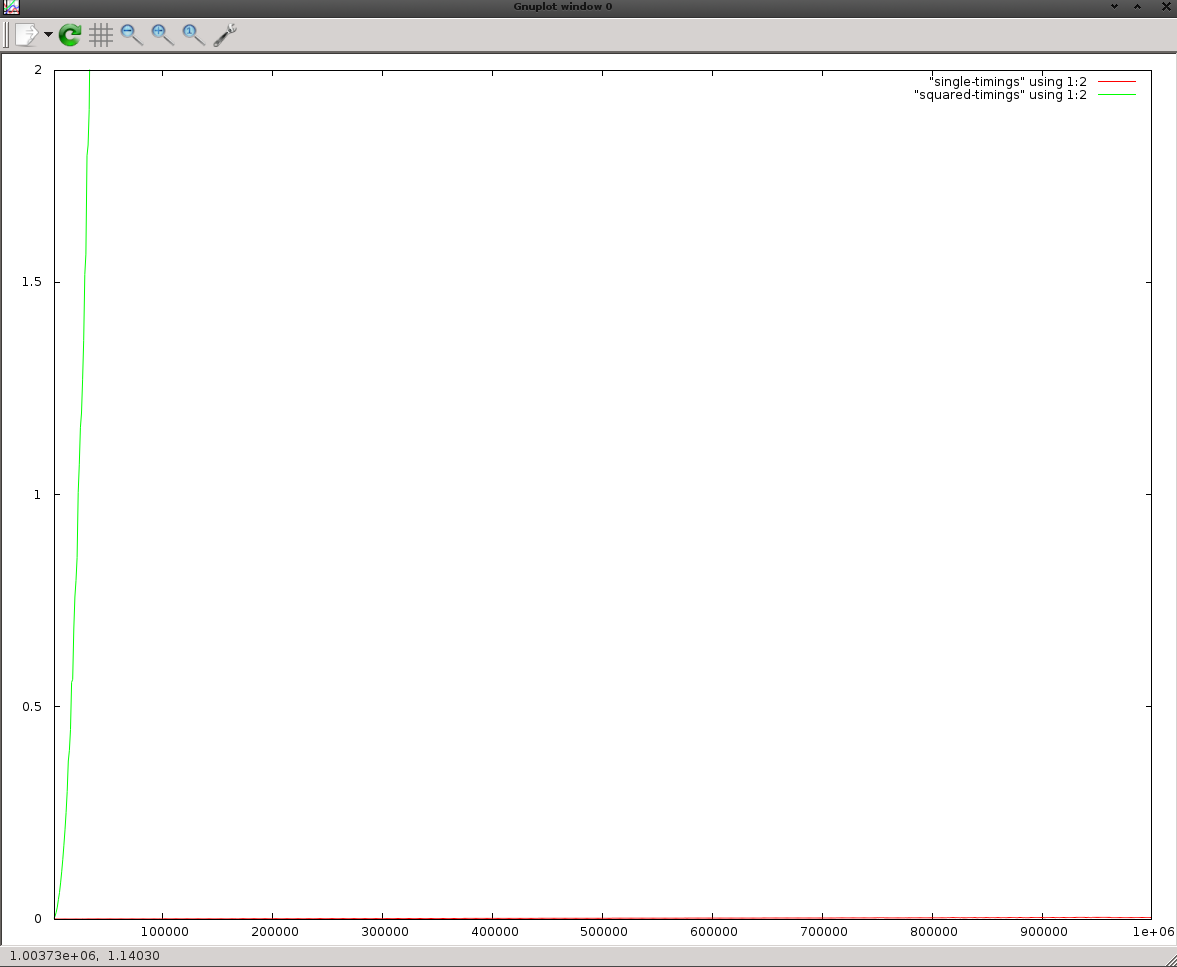
\includegraphics[width=1.0\textwidth]{../imgs/timing-gotcha2.png}
}
\end{columns}
\end{frame}

%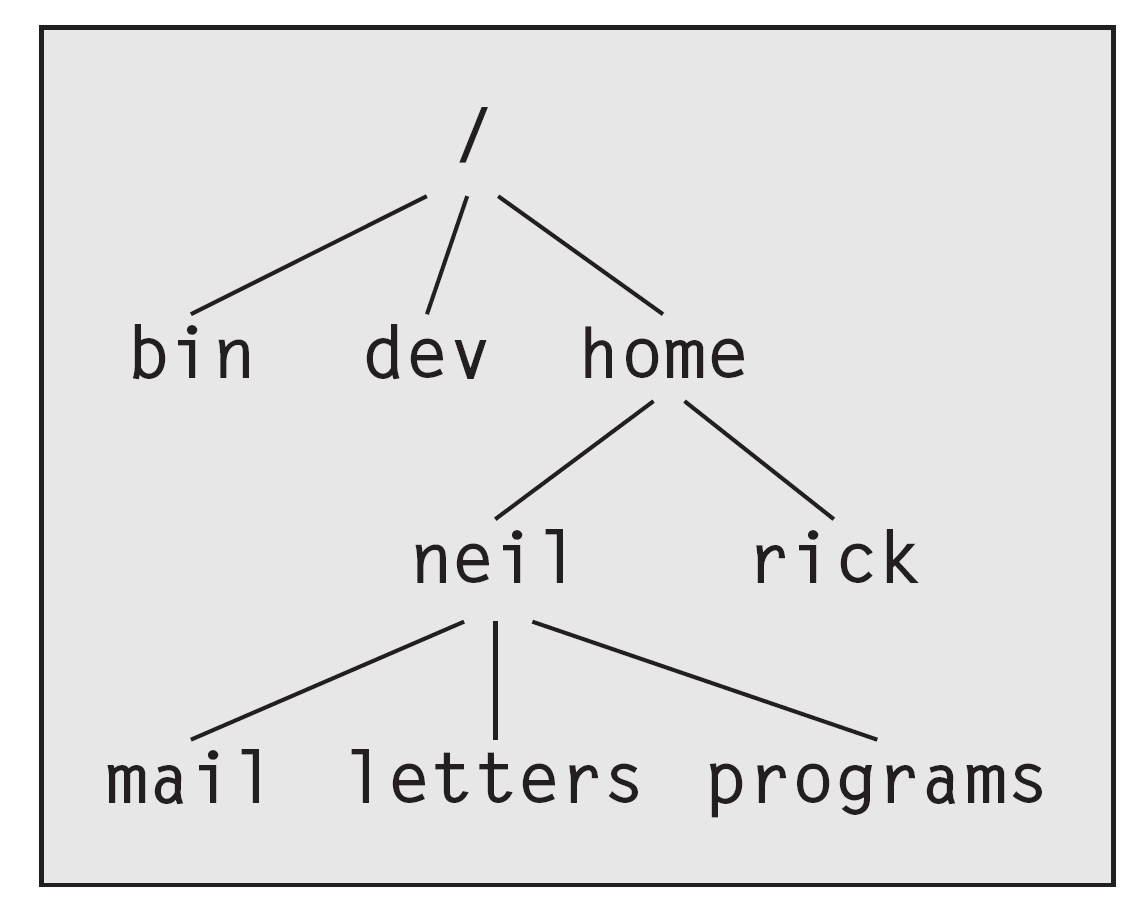
\includegraphics[width=1.0\textwidth]{../imgs/simple-directories.png}

%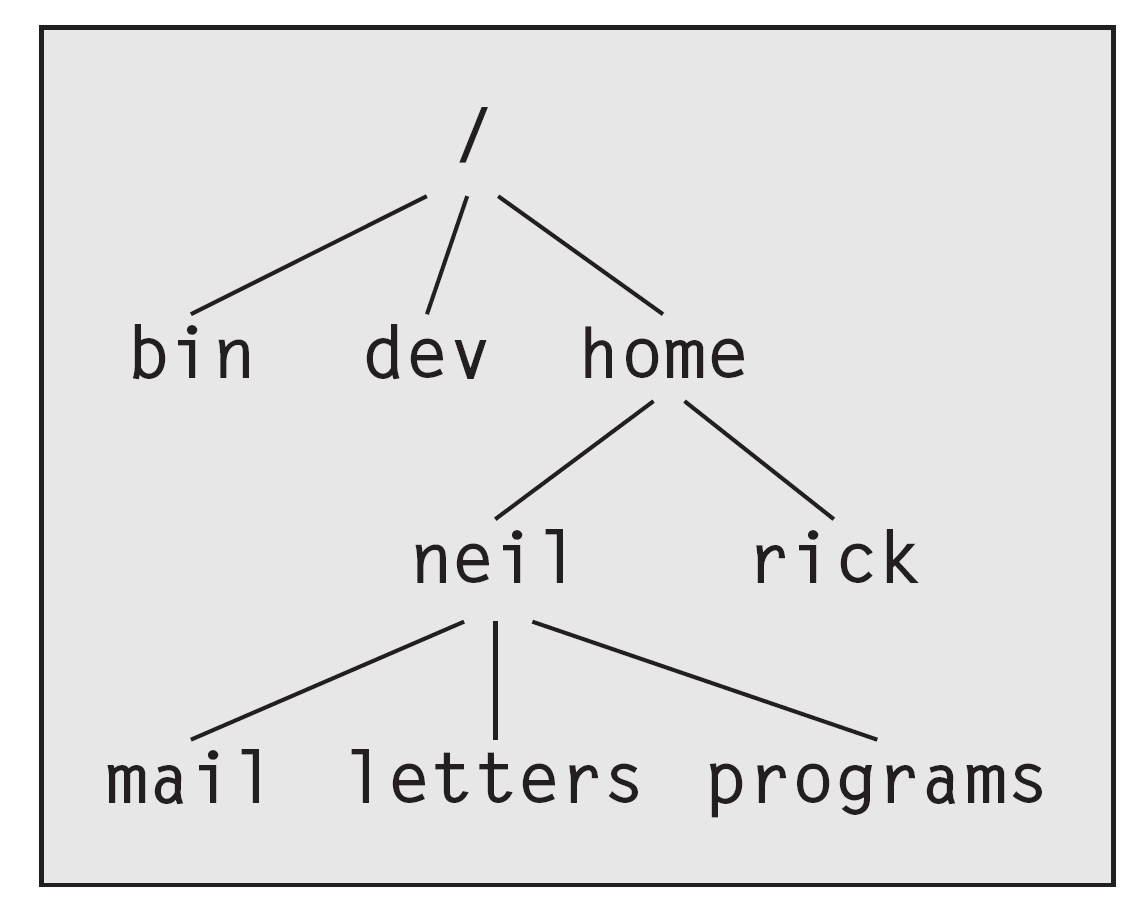
\includegraphics[width=1.0\textwidth]{../imgs/simple-directories.png}
\begin{frame}{Performance Tips}
\begin{itemize}
\item Make sure you are working on optimizing the correct function and looking for the correct code improvements.
\item From our example:\\
%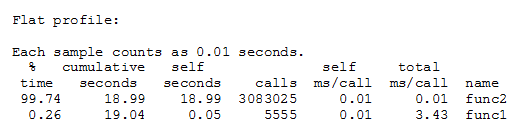
\includegraphics[width=1.0\textwidth]{../imgs/prof3.png}
\includegraphics[width=1.0\textwidth]{../imgs/perf.png}
\item Most of the time is spent in sumOfOneTo, so improving sumOfOneTo's performance may help.
\item Improving performance of sumOfOneToSquared would not help that much.
\begin{itemize}
\item Maybe we can memoize past results to use in the future -- or use a better data structure.
\end{itemize}
\end{itemize}
\end{frame}

\section{Conclusion}
\subsection{}

%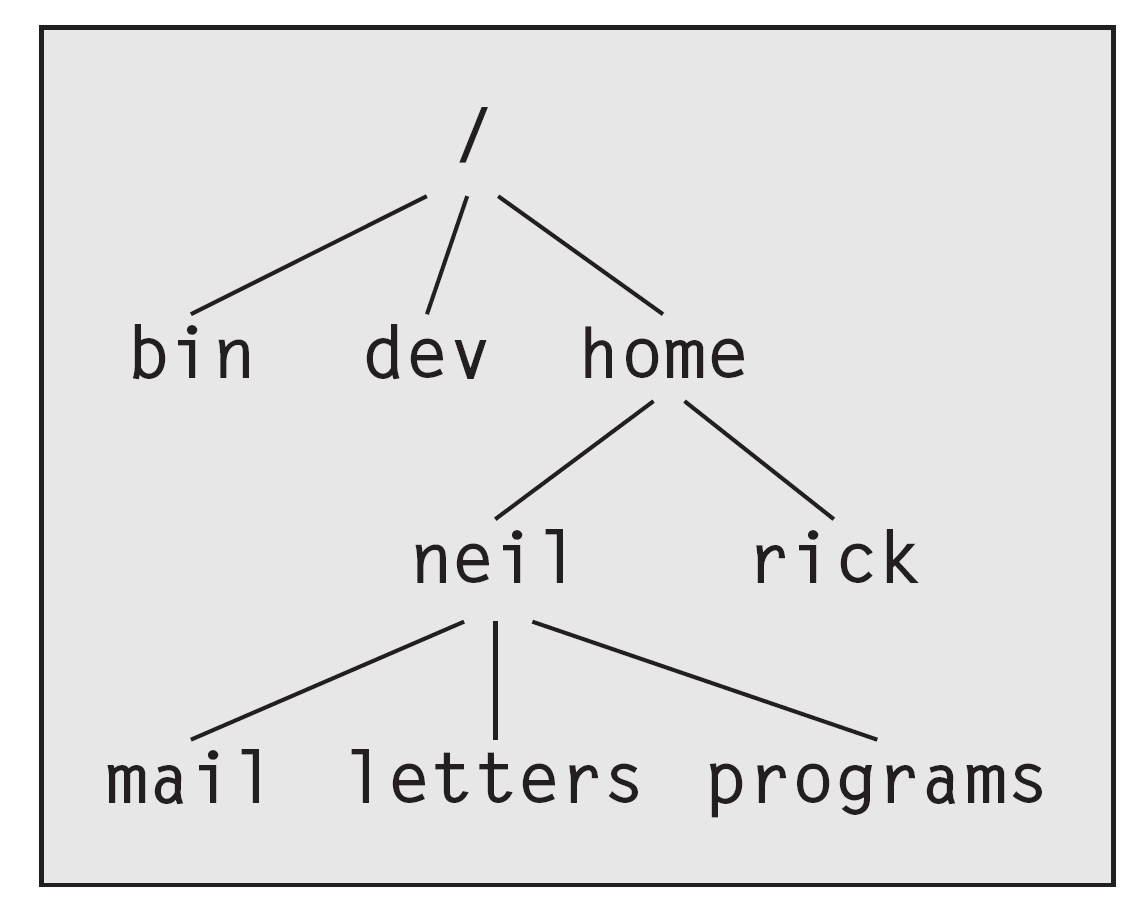
\includegraphics[width=1.0\textwidth]{../imgs/simple-directories.png}
\begin{frame}{Summary}
\begin{itemize}
\item Again, there is a lot and we are scratching the surface.
\item Important outcomes:
\begin{itemize}
\item Be able to analytically deduce the performance of code.
\item Be able to profile code to find the hot spots.
\item Be able to emperically run programs to evaluate performance.
\item Understand there are anomalies that will not be addressed in this class.
\end{itemize}
\end{itemize}
\end{frame}

\end{document}
